\documentclass[longbibliography,nofootinbib]{revtex4-1}

\newcommand{\kms}{NuCypher}

\usepackage{listings}
\usepackage{graphicx}
\usepackage{amsmath}
\usepackage{subcaption}
\usepackage[labelformat=parens,labelsep=quad, skip=3pt]{caption}
\usepackage[margin=5pt]{subfig}
\usepackage[usenames]{color}

\renewcommand{\baselinestretch}{1.4}
\setlength{\parskip}{1em}
\definecolor{darkgreen}{rgb}{0.00,0.50,0.25}
\definecolor{darkblue}{rgb}{0.00,0.00,0.67}
\newcommand{\figref}[1]{Fig.~\ref{#1}}
\usepackage[breaklinks,pdftitle={NuCypher: a proxy re-encryption network to empower privacy in decentralized systems}, pdfauthor={Arjun Hassard},colorlinks,urlcolor=blue,citecolor=darkgreen,linkcolor=darkblue]{hyperref}
\graphicspath{{pdf/}}

\usepackage[T1]{fontenc}
\usepackage{lmodern}
\lstset{
    basicstyle=\ttfamily,
    basewidth={0.5em, 0.5em},
    columns=fullflexible,
}

\begin{document}

\title{NuCypher Network: Staking Protocol \& Economics}

\author{Michael Egorov}
\email{michael@nucypher.com}
\author{MacLane Wilkison}
\email{maclane@nucypher.com}
\author{Arjun Hassard}
\email{arjun@nucypher.com}
\affiliation{NuCypher}

\begin{abstract}
This paper describes the protocol mechanisms which aim to incentivize and sustain reliable supply participation in the NuCypher network, including the regular distribution of a subsidy to actively staking service-providers. The subsidy is generated through the scheduled growth of the native token's circulating supply, following a `two-phase' model designed to maximize service quality, node operation efficiency and network decentralization. The paper also explains the relationship between discretionary stake configurations and subsidy size; in particular, extra incentives to commit to longer staking durations. The rules for stake management, including locking, unwinding, and withdrawing, are covered in detail, and the impact of these service-provider decisions on the global supply is deduced. Finally, an analysis of historical service-provider behavior in existing staking networks provides an empirical context for design and parameter choices.
\end{abstract}

\date{\today}
\maketitle

\section{Motivation \& Context}

The Nucypher network is an example of a \textit{decentralized service marketplace}, providing infrastructural services to digital applications/systems (`users') via a distributed supply of independent node operators (`service-providers'), who run the same software but have discretion over certain service parameters. NuCypher's primary offerings, secrets management and dynamic access control, are a breed of scaleable, trust-minimizing, censorship-resistant services – the strength of each value proposition depending, to some extent, on long-term commitment to the network by a large, diversified population of service-providers. Aspects of the NuCypher service necessitate concurrent work by multiple service-providers to be maximally secure and redundant.
\\\\
Hence, like many decentralized service marketplaces, and indeed centralized marketplaces, it is critical to the NuCypher network that supply is abundant and reliable – and that the network establishes this state prior to the emergence of user adoption, lest the adoption be short-lived. As with any network, operating a node incurs various overheads, upfront and ongoing, and denominated in fiat, cryptocurrency and time. Moreover, eligibility for service provision in the NuCypher network is contingent on the acquisition and time-locking of collateral (`staking'), which burdens the service-provider with ongoing risk and opportunity cost.
\\\\
If demand for NuCypher services rise sufficiently, direct payments from users (`fees') will sustain the operations of service-providers. However, before demand reaches this threshold, another stream of revenue is required – to incentivize a sufficient number\footnote[1]{The number of independent service-providers is approximately proportional to the level of security, redundancy and censorship-resistance available to users, but these benefits begin to plateau at roughly >500 service-providers.} of service-providers to join the network, and to subsidize the cost of their operations until a mature fee market materializes. Thus, a vitally important mechanism in the NuCypher protocol is the predictable distribution of subsidies to actively staking service-providers, realized through the growth of the native token's circulating supply. 
\\\\
The NuCypher protocol's \textit{monetary policy} – the design choices and parameters that govern this subsidy mechanism – is the primary focus of this paper. 

\section{Two-phase Subsidy Model}

\subsection{Overview}

\subsubsection{Basic Properties}
From the moment the NuCypher network launches, the protocol will distribute a daily subsidy, exclusively to actively staking service-providers. The size of subsidy will be proportional to the relative size of the stake\footnote[2]{The quantity of user requests (`work') delivered to service-providers, and therefore exposure to fee-earning opportunities, is also proportional to the relative size of their stake.}. Service-providers will be further incentivized to commit to longer spans of service provision through a commensurate subsidy, and to increase their stake size with the subsidies they receive (`re-staking'). The genesis supply – the number of tokens circulating at network launch – will be 1 billion tokens. Over the course of the network's lifetime – as $t$ approaches $\infty$ – the circulating supply will approach a maximum of roughly 3.885 billion tokens.

\begin{figure}[h!]
    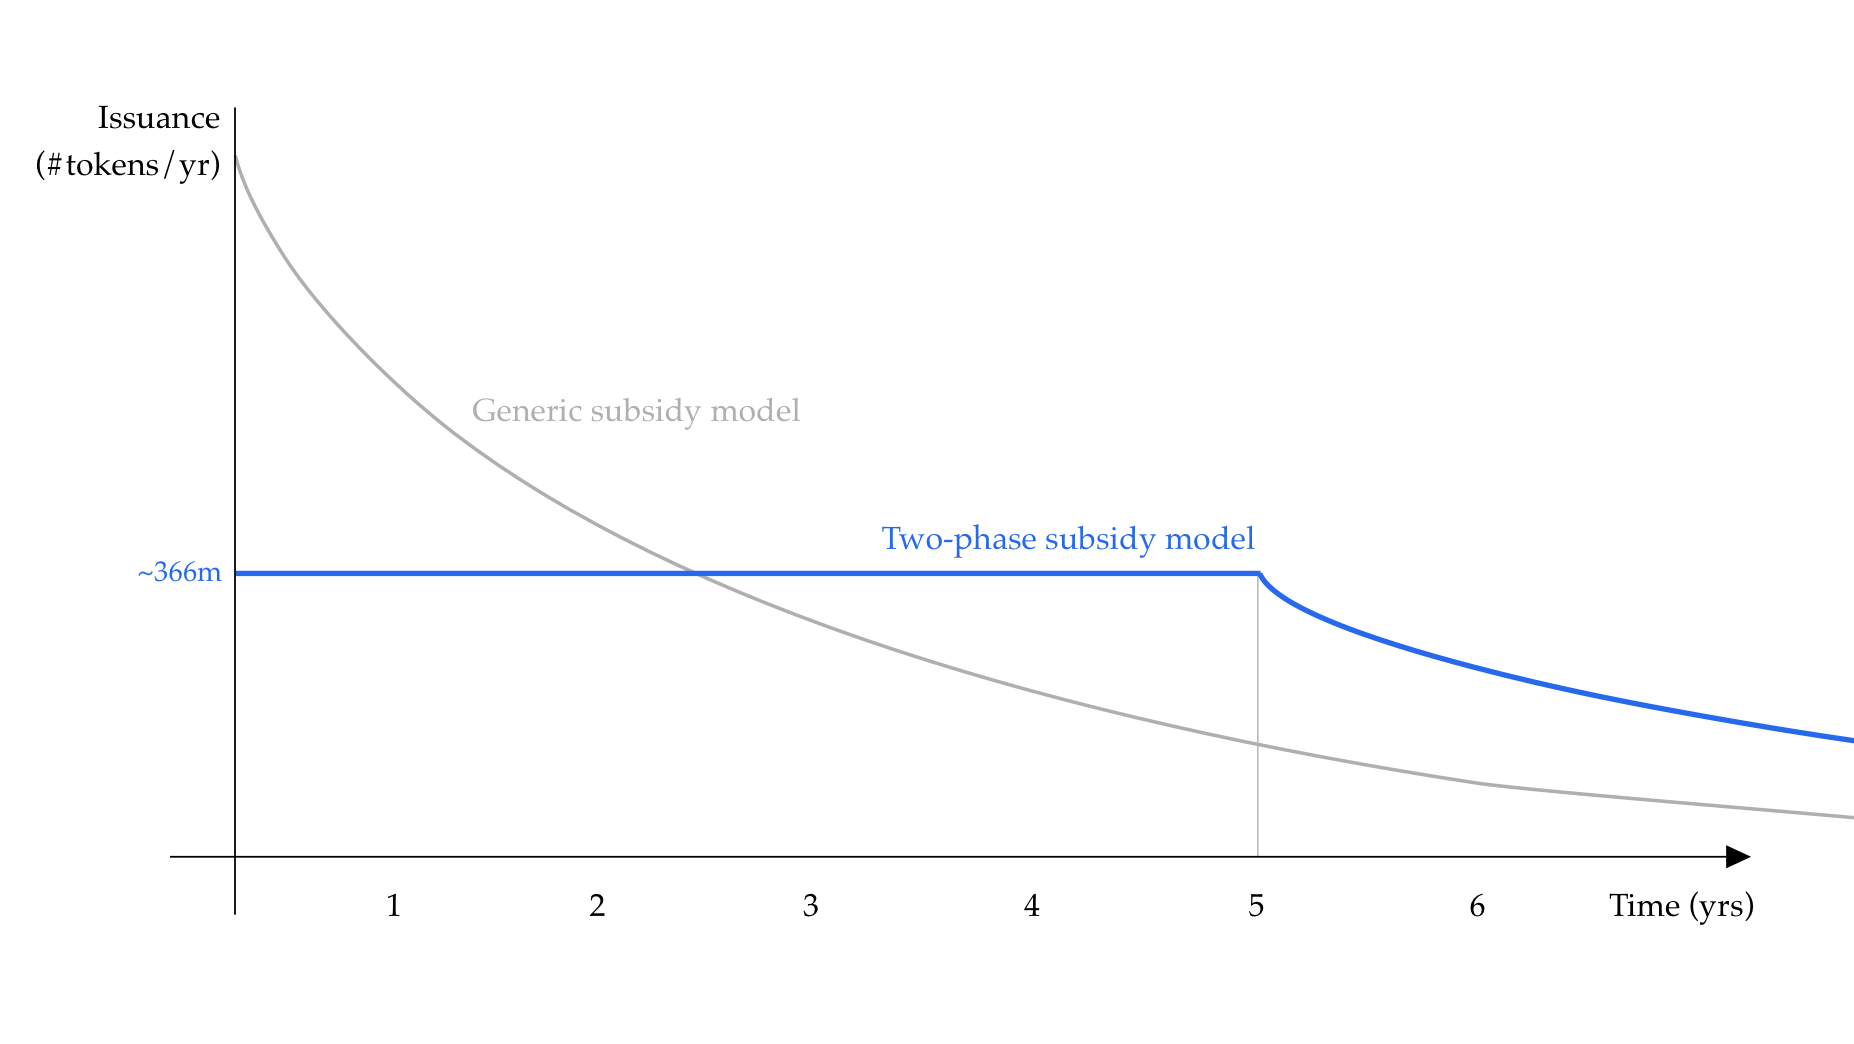
\includegraphics[width=0.8\textwidth]{Two_phase_model.png}
    \caption{Illustrative comparison of the two-phase model with a popular subsidy schedule. Note that the y-axis refers to an absolute figure of tokens, as opposed to an `inflation rate'.}
    \label{fig:tp}
\end{figure}

\subsubsection{Phase 1 – Constant Issuance}
In a notable divergence from prevailing subsidy models, NuCypher does not administer a decreasing subsidy in the first few years of the network's existence. Instead, the NuCypher protocol enforces a more \textit{temporally equitable} model, in which, all things equal, the subsidy a service-provider receives remains a constant size for at least the first five years of the network's existence. In this phase (`Phase 1'), a maximum of 366 million new tokens will be minted and distributed annually, equivalent to expanding the circulating supply by a maximum of 1,002,509 tokens every period (days). 
\subsubsection{Phase 2 – Decaying Issuance}
Phase 2 commences as soon as the circulating supply reaches a total of 2,829,579,800 tokens – the earliest the protocol can enforce the phase switch is 5 years after network launch. In Phase 2, fewer tokens will be minted in each successive period, such that the daily minting figure decays exponentially with a minimum half-life of 2 years. 

\subsubsection{Variable issuance}
In the NuCypher protocol, global issuance is modified by the average stake lock-up duration, but for the sake of simplicity this paper initially discusses a scenario in which all node operators choose a lock-up of 12 months or longer. In reality, the average stake lock-up duration is likely to be lower, which would imply fewer total tokens minted per period in both phases. Regardless, lock up durations are chosen entirely at the service-provider's discretion, and hence they retain control the size of subsidy received. Variable issuance has an impact on the global economy and the moment in which the protocol switches from Phase 1 to Phase 2, covered in section III (Staking Protocol). 

\subsubsection{Note regarding `inflation rates'}

Decentralized network monetary policy often makes reference to a so-called `inflation rate'. In this model, since Phase 1 sees an constant amount of tokens minted in each period, the effective rate at which the circulating supply grows will decrease period-to-period (and year-to-year). In Phase 2, the number of tokens minted per day decreases, which accelerates the decline in the supply growth rate. Stakes generally also experience a decreasing growth rate, the magnitude of which is heavily affected by discretionary stake configurations. To avoid misleading terminology, this paper does not refer to a rate, instead using \textit{issuance} as a short-hand for the absolute sum of tokens minted per period.

\subsection{Rationale for two-phase model}

\subsubsection{Demand uncertainty}\label{demand}

These demand-related premises form the basis for the two-phase model: 
\begin{enumerate}
\item There is little certainty regarding the length of time that will elapse between the network's launch and the development of meaningful demand from users (developers, end-users \& others).
\item This early-stage demand is particularly fragile, because new users are naturally more fickle. Specifically, neither developers nor their end-users have compelling reasons to tolerate an inadequate service (e.g. too few service-providers available to manage a sharing policy), such as the sunk costs of integration, reliance on the service, or other forms of path dependency, all of which are more likely to play a role later in the network's lifetime. Early users are unavoidably required to take a greater risk than later adopters, as they do not have the experience of existing customers as evidence of a reliable or valuable service.
\item Many existing subsidy models involve daily token issuance dropping exponentially [ADD REFERENCE], right from launch. However, if the network's fee market does not reach a sufficient stage of maturity in time to make up for this sharp reduction in subsidy, some node operations may be rendered entirely unsustainable. 
\item Most importantly, some early adopters will come to NuCypher with a use case that inflexibly requires long-lasting sharing policies. This means that the protocol must motivate the successive re-commitment to long token lock durations (i.e. staking for 12+ months) by a sufficient population of service-providers. A diminished subsidy, in lieu of a mature fee market, may not be enough to incentivize this repeated and essential re-commitment. 
\end{enumerate}

\\\\
Hence this model attempts to mitigate the risk of \textbf{fledgling network demand coinciding with a disincentivized, dwindling or transient supply} of service providers. Note that these arguments do not involve strong claims about when (or if) network adoption will occur. Instead, it is the acknowledgement of uncertainty with respect to an adoption timeline that forms the core of the problem, and underpins the utility and advantage of a stable issuance phase as part of a two-phase minting schedule. 

\subsubsection{Impeding centralization}

A constant issuance in Phase 1 brings other benefits, including the partial mitigation of a centralizing dynamic suffered by many staking networks, in which larger service-providers utilize subsidies to increase/consolidate control of the token supply, thanks to the allocation of tokens in proportion to stake size [ADD REFERENCE]. Moreover, larger service-providers can re-stake a greater percentage of subsidies (not needing to convert as much to fiat to cover operational costs), precipitating a `rich-get-richer' dynamic. If token issuance is highest in the earliest days of the network, larger service-providers are granted an even greater head-start over new service-providers who start staking in a later era, \textbf{the presence of whom provides the network with an important, long-term counter-balance against centralization}. Relatedly, an important rationale for the \textit{work token} model is the supposition that new service-providers purchase the network's native token in order to stake and earn revenue [ADD REFERENCE]. With a token issuance that decays from genesis, late-joining service-providers are doubly disadvantaged – they must pay the market price to acquire tokens, plus they receive a diminished subsidy. 
\\\\
Consequently, a two-phase subsidy model assists all would-be service-providers who don't happen to stake right at network launch but decide to do so at a later date. By addressing the temporal inequity of immediately decreasing issuance, we impede problematic centralization trends.

\subsubsection{Risks to operational feasibility, incentives and pricing}

As illustrated in figure 1, generic subsidy models comprise a high issuance at genesis and in the first few years of the network's existence. Setting the peak issuance (the maximum number of tokens minted per day) at a comparatively lower figure may address the following problems: 
\begin{itemize}
\item The greater the real-world value of the subsidy, the further from a fee-driven `reality' a service-provider's set-up may be in economic terms (for example, in terms of operational efficiency). When subsidies eventually run out, service-providers who are unable to adapt may cease operations, threatening general service availability or even reneging on existing commitments to users. Under a model with higher token issuance early on, these inefficient operations may control a substantial proportion of the circulating supply by this point. 
\item If subsidies are worth significantly more than the typical sum of transaction fees earned in the same period, then the incentive to earn those fees may be blunted. This is particularly problematic for the protocol if the work required to collect subsidies does not align well with work required to earn fees, and the reliability of the latter impacts overall service quality. 
\item High but decreasing subsidies may compel some service-providers to offer an unsustainably cheap service, with the intention of raising prices later once subsidies dry up. Any developers and their end-users that have become reliant on the service, but are unable to afford the higher price point, may see their application/business thrown into jeopardy. The existence of this risk is a serious friction for would-be network users planning an integration and justifying the associated upfront costs and technical dependency.
\item In NuCypher's case, existing market prices for comparable services – key/secrets management and dynamic access control – are extremely low on a per-user basis. Profitability is generally achievable through high volume, which is a long-term endeavour. This business reality aggravates all three above issues described in this sub-section.
\end{itemize}

\subsection{Parametrizing the Two-Phase Model}

\\\\
 In order to parametrize the two-phase model, we select certain invariants, and derive the other parameters from those constraints. We fix the total number of tokens ever to be minted, $S(\infty)$ at approximately 3.885 billion, and the half-life of the issuance decay in the second phase, $T_{1/2}$, at 2 years. The genesis supply ($S_0$) is 1 billion tokens. Note that some numerical figures in this section are rounded for readability.
\\\\
The most important parameter for this subsidy schedule is the maximum number of tokens minted per period during the first phase, which we describe as the `max issuance' ($I_{max}$). Using an axiom for $S(\infty)$, we can derive $I_{max}$. $S(\infty)$ is the sum of (1) the tokens circulating at genesis, (2) the tokens minted in Phase 1, and (3) the tokens minted in Phase 2. Note that we initially express $I_{max}$ as a percentage of the genesis supply per year, before converting it to an absolute number of tokens per period – see equation 7.

\begin{equation}
    S(\infty) = S_0  +  S_0 \cdot \int_0^{5} I_{max}(t)\, dt  +  S_0 \cdot \int_0^{\infty} I(t)\, dt
\end{equation}
\\
Note that we use 5 years as a provisional duration for Phase 1 in order to calculate the maximum possible issuance. In practice, the issuance will be lower, and hence the switching of phases ($T_{1\rightarrow2}$) will likely occur at $t$ > 5 years – see equation 12. Note also that the boundaries of the second integral are $0$ and $\infty$, rather than $5$ and $\infty$, because the issuance curve in Phase 2 is computed independently of Phase 1. In Phase 2, the decaying issuance at a time $t$ is a function of $I_{max}$, since it commences at this figure.
 
\begin{equation}
    I(t) = I_{max} \cdot 2^{-\frac{t}{T_{1/2}}}
\end{equation}
\begin{equation}
    3.885 \cdot S_0  = S_0 + S_0 \cdot \int_0^{5} I_{max}(t)\, dt + S_0 \cdot \int_0^{\infty} I_{max} \cdot 2^{-\frac{t}{T_{1/2}}} \, dt ,\\
\end{equation}
\begin{equation}
    3.885 = 1 + 5 \cdot  I_{max} + I_{max} \cdot \left[\frac{-2^{(1-\frac{t}{2})}}{\ln{2}}\right]_0^\infty .\\
\end{equation}

\begin{equation}
    2.885 = I_{max} \cdot (5 + \frac{2}{\ln{2}})
\end{equation}

\begin{equation}
   I_{max} = \frac{2.885}{7.885} = 36.6\%
\end{equation}
\\
We multiply by $S_0$ and convert $I_{max}$ into the absolute number of tokens minted per period.

\begin{equation}
    \label{eq:abs}
   \frac{I_{max} \cdot S_0}{365} = 1,002,509\:\:new \:tokens \:per \:period
\end{equation}

Hence, the two-phase schedule sees a maximum of 1,002,509 tokens minted every period until there are 2,829,579,800 billion tokens in the circulating supply. At this point the protocol will switch to Phase 2, in which a further 1,055,810,282 tokens will be minted until t = $\infty$.


\section{Staking protocol}

\subsection{Subsidy size and commitment time}

\subsubsection{Sub-stakes}

In order to be eligible to answer user requests, earn fees, and receive subsidies, a service-provider must commit to servicing the network for some period of time by locking collateral (staking). Service-providers specify a stake unlocking time in the future $t_1$, where at time $t$ the minimum duration $t_1 - t$ may not be fewer than $D_{\min}$ = 31 periods, but may be any greater number of periods .
\\\\
The NuCypher protocol allows service-providers to partition their stake into sub-stakes, up to a maximum of 30. A sub-stake has a unique remaining duration $D$ – the number of periods until it unlocks and the tokens become freely withdrawable. The sub-stake size $\theta$ is the number of tokens locked. It is possible to extend (but not reduce) $D$ for a sub-stake, or split a sub-stake by extending $D$ for part of it. It is also possible to acquire more tokens and increase $\theta$ in any sub-stake.

\begin{figure}[h!]
 \centering
    \begin{minipage}{0.48\textwidth}
        \centering
        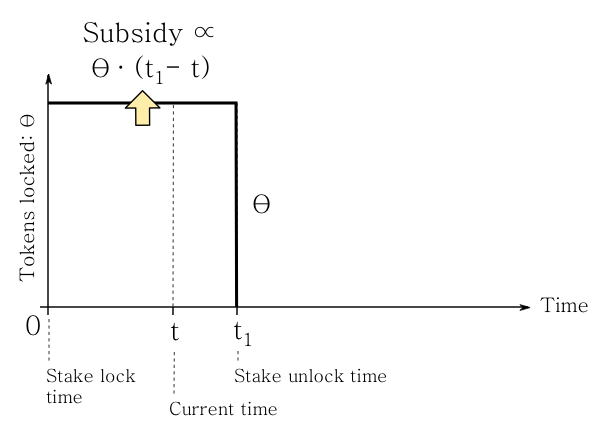
\includegraphics[width=0.99\textwidth]{graphs/one-step.png}
        \caption{A single stake which unlocks at time $t_1$. The stake receives a subsidy proportional to its size ($\theta$) and remaining duration to unlock ($D = t_1 - t$).}
    \end{minipage}\hfill
    \begin{minipage}{0.48\textwidth}
        \centering
        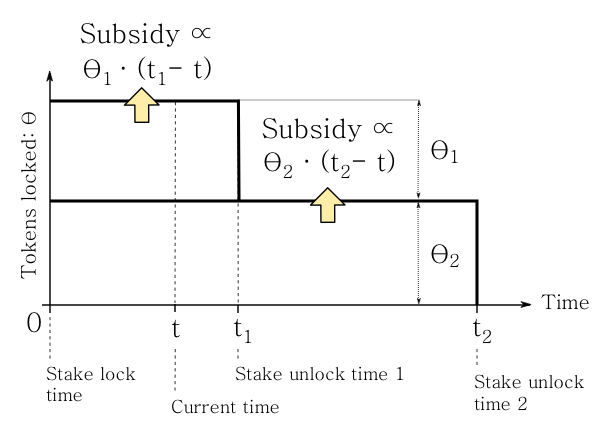
\includegraphics[width=0.99\textwidth]{graphs/two-steps.png}
        \caption{The stake in figure 3 has been split into two sub-stakes. This was achieved by extending the duration to unlock ($D_2 = t_2 - t$) for a portion (of size $\theta_2$) of the total tokens in the original stake. The two sub-stakes will receive differently sized subsidies.}
    \end{minipage}
\end{figure}

\subsubsection{Subsidy coefficient}

Secrets management and dynamic access control, the primary services offered through NuCypher, require service-providers to securely hold re-encryption keys and respond to access/revocation requests until the associated sharing policies expire. This involves maintaining a unique state on behalf of each user, which must persist without fail until the specified expiration – which in some use cases will not transpire for extended periods of time (12 months or longer). To ensure that service-providers stick around to perform these duties, the economic security of locked collateral must persist for at least as long as the sharing policies are active. Hence, the NuCypher protocol must further incentivize service-providers to lock their sub-stakes for as long as possible.
\\\\
As shown in figures 3 \& 4, the size of subsidy earned by each sub-stake $i$ is proportional to the duration of time until it unlocks ($D_i = t_i - t$), and the number of tokens in the sub-stake ($\theta$). Sub-stakes that unlock in 1 year or more receive the maximum subsidy ($\kappa=1$), whereas a sub-stake that unlocks in 1 month would receive slightly over half the maximum subsidy ($\kappa\approx0.54$). The subsidy coefficient $\kappa$ for a given sub-stake $i$ is calculated as following, where $D_{max}$ is currently set to 1 year or 365 periods:
\begin{equation}
    \kappa_i &=& \left(0.5 + 0.5 \cdot \frac{\min(D_i, D_{max})}{D_{max}}\right)
\end{equation}

In Phase 1, a sub-stake $i$ of size $\theta$ will receive the following subsidy, where $\Theta$ is the sum of all locked sub-stakes and $I_{max}$ is the maximum number of tokens that can be minted in a period $p$:

\begin{equation}
    \label{eq:ds}
    ds_{\theta i,p} = \kappa_i \cdot \frac{\theta_i}{\Theta} \cdot I_{max} 
\end{equation}

In Phase 2, a sub-stake $i$ of size $\theta$ will receive the following subsidy, where $S(\infty)$ is the total number of tokens ever to be minted (roughly 3.885 billion), $S_{p-1}$ is the circulating supply in the period before $p$, and $T_{1/2}$ is the issuance decay half life:

\begin{equation}
    \label{eq:rate-max}
    ds_{i,p} = \kappa_i \cdot \frac{\theta_i}{\Theta} \cdot \frac{\ln{2}}{T_{1/2} \cdot 365 } \cdot \left[S(\infty) - S(p-1) \right]\\
\end{equation}

\subsection{Variable issuance and the global economy}

The circulating supply at a given period $p$ is the sum of the tokens received thus far by all sub-stakes (this does not include the genesis supply):
\begin{equation}
    dS_p= \sum_i ds_{i,p}
\end{equation}

Sub-stakes locked for a short times earn less than the maximum subsidy, thereby slowing the expansion of the entire circulating supply – tokens are only minted if they are to be distributed to node operators. The implication of any instance of $\kappa$ < 1 is that it will take longer than the provisional 5 years to mint all the tokens reserved for Phase 1. The year in which the protocol switches from the first to second phase ($T_{1\rightarrow2}$) is therefore: 

\begin{equation}
\label{phaseswitch}
    T_{1\rightarrow2}= \frac{S_{Ph1}}{S_0 \cdot \kappa^* \cdot I_{max}}
\end{equation}
\\
Where $\kappa^*$ is the average lock duration of all sub-stakes, weighted by relative size, and $S_{Ph1}$ is the total number of tokens reserved for Phase 1, excluding the genesis supply (roughly 1.83 billion). For example, if $\kappa^*$ were to equal 11 months, $T_{1\rightarrow2}$ would be  5 years and 79 days. The longest Phase 1 can last (i.e. if all sub-stakes unlock in 1 month or less, so $\kappa^* \approx 0.54$), barring changes to the protocol, is 8 years and 209 days.

\begin{figure}[h!]
    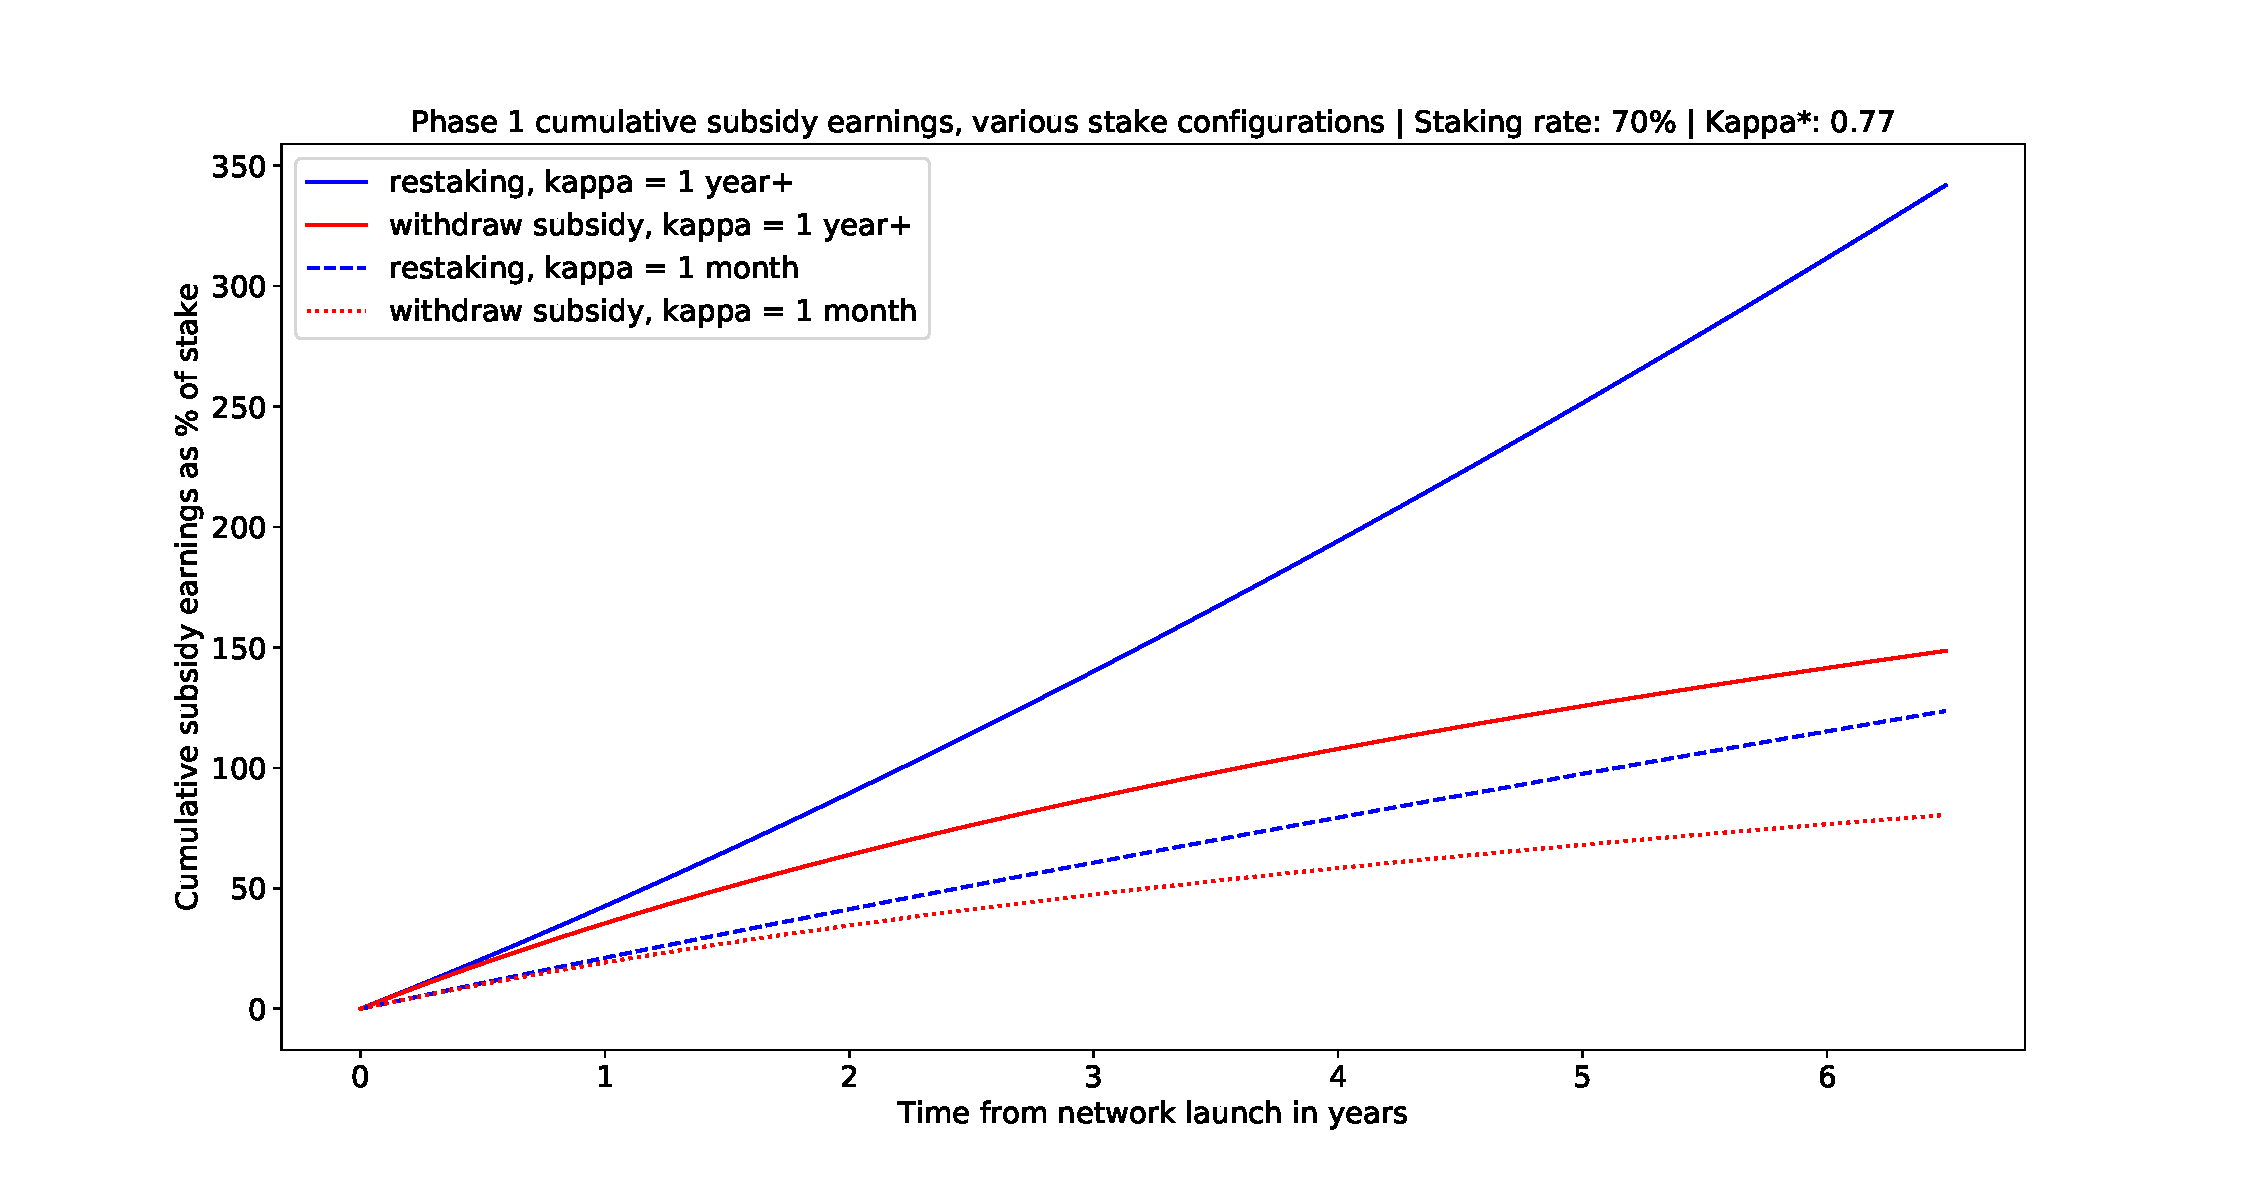
\includegraphics[width=\textwidth]{graphs/SubsidyP1.pdf}
    \caption{Cumulative total subsidies received in \textbf{Phase 1}, for stakes unlocking in 12+ and 1 month, and configured to re-stake or withdraw subsidies. Staking rate \& average lock duration assumed to be 70\% and 0.77 respectively.}
    \label{fig:tp}
\end{figure}

\begin{figure}[h!]
    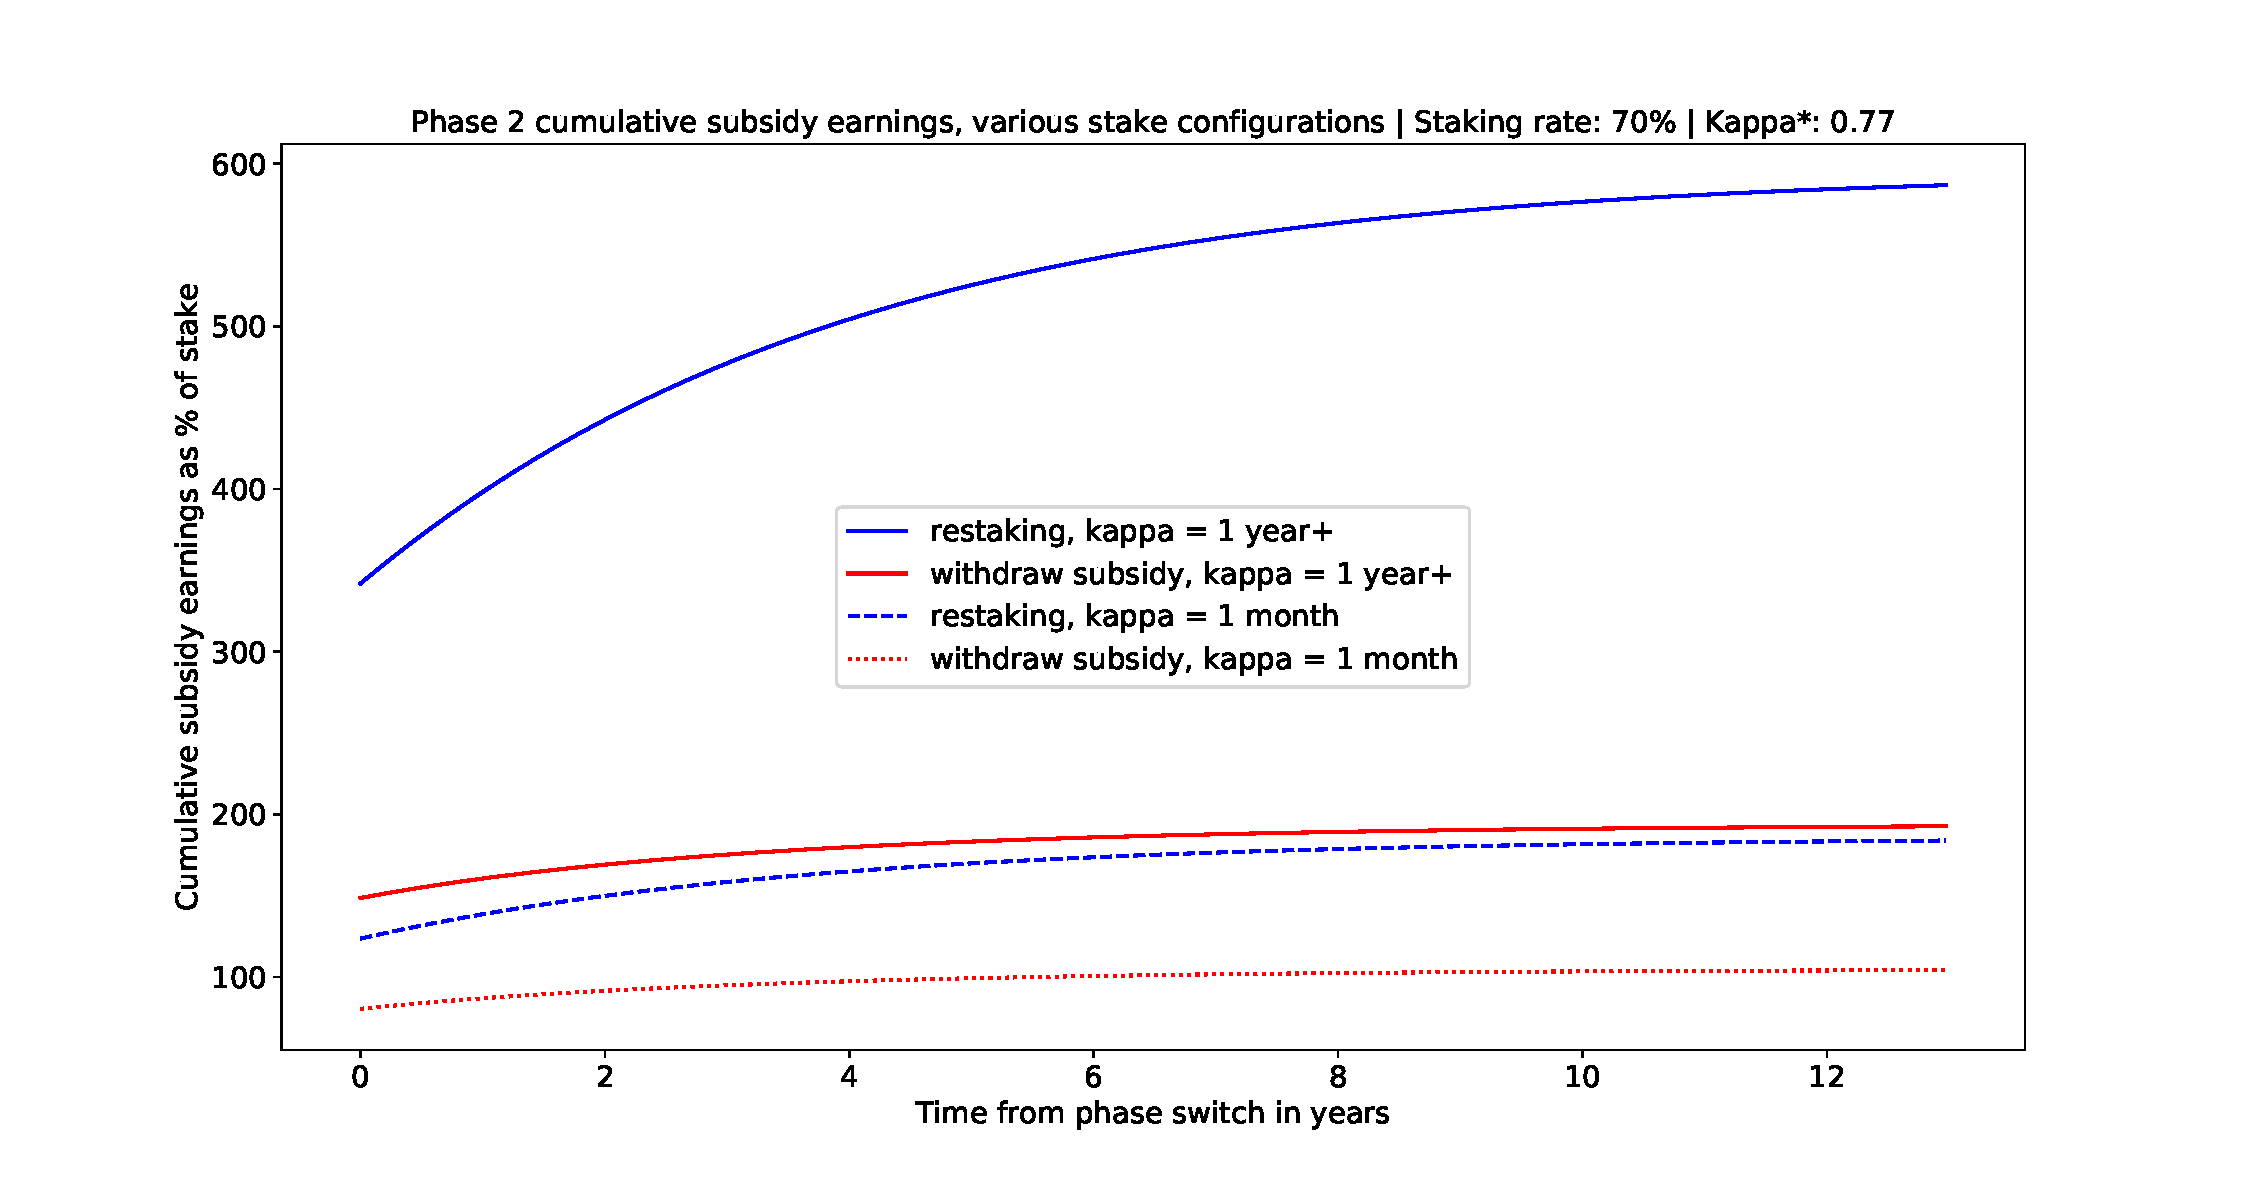
\includegraphics[width=\textwidth]{graphs/SubsidyP2.pdf}
    \caption{Cumulative total subsidies received in approx. first 7 years of \textbf{Phase 2}, with all other parameters the same as figure 4. Note that all totals at the end of Phase 1 equal those at the start of Phase 2.}
    \label{fig:tp}
\end{figure}

\subsection{Other considerations for service-providers}

\subsubsection{Re-staking}

A service-provider is free to withdraw the subsidies their sub-stakes receive. If they pocket all incoming tokens, then their sub-stakes will remain the same size, but are likely to decrease as a fraction of the total tokens staked ($\Theta$), which means their period-to-period subsidy, and exposure to user requests, will also decrease. 
\\\\
A service-provider may re-stake their subsidies, provided they have the capacity to support the potential increase in workload (user requests). If the sub-stakes in question are set to unlock in 1 year or longer, and the average lock duration is shorter than this, then re-staking all subsidies would see those sub-stakes grow and account for a increasing fraction of the total tokens staked. As a result, the subsidies received would also rise over time. \\\\
The dramatic difference in long-term  cumulative earnings between various staking strategies over both phases is shown in figures 4 and 5. 

\subsubsection{Winding down sub-stakes}

The default setting for all sub-stakes is for $t_i$, the stake unlock duration, to be automatically prolonged. This keeps the subsidy coefficient ($\kappa$) constant. If a service-provider proactively initiates a wind-down – that is, they specify an unlock date in the future for a sub-stake, then the corresponding subsidy will continually decrease as the time to unlock gets smaller and smaller, until $\kappa$ reaches a minimum of $0.5$.

\subsubsection{Staking rate \& real yield}

The \textit{staking rate} is the percentage of tokens staked out of the total circulating supply in a given period. Other protocols refer to this variable as the `participation rate' or `total staked'. The \textit{real yield} is used to describe the true subsidy earnings of actively staking service-providers at a given timestamp, accounting for the staking rate and dilution. The real yield is a function of the nominal issuance (or `inflation rate' in other networks). The real yield is usually expressed as a percentage of stake size, and on an annual basis. Other protocols refer to this variable as the `adjusted reward' or simply `yield'. 
\\\\
The NuCypher protocol distributes subsidies such that the real yield $Y_r$ in a given period is inversely proportional to to the staking rate $\lambda$: 

\begin{equation}
    Y_r \:\:\alpha\:\: \frac{I_{max}}{\lambda}
\end{equation}

For example, the calculations for figures 4 and 5 assume a constant staking rate of 70\%.

\section{Empirical analysis of existing networks}

\textit{Full study to be published. This section summarizes analysis thus far and evaluates results with respect to the two-phase model.}

\subsection{Outline}

\subsubsection{Objectives \& Data Characteristics}

The objective of this analysis is to better understand the relationship, if any, between (1) the variable real value of a subsidy received by service-providers/stakers (the \textit{real yield}), and (2) their subsequent, collective decision to increase, decrease or maintain the size of their stake, expressed as a percentage of the total circulating tokens (the \textit{staking rate}). This pertains directly to the primary objective of the NuCypher staking protocol mentioned in section 1 – to maximise the abundance and reliability of network supply – which is reflected in the health\footnote{`Health' in this context simply means the percentage of tokens staked – for example, a network with only 5\% of tokens staked might be described as unhealthy, because it may be highly centralized and/or not have the capacity to deal with demand} and stability of the staking rate. This study employs data sets from two independent sources, (A) Staking Rewards and (B) Yields:
\\\\
(A) Staking Rewards provides data on the networks Tezos, Cosmos, Livepeer and Irisnet. The Staking Rewards time series is 4x daily (every 6 hours) and runs from February 2019 (Livepeer), March 2019 (Cosmos, Irisnet) and July 2019 (Tezos) until February 2020 (all four networks). Variable (1) is referred to as the \textit{adjReward}, and variable (2) as the \textit{totalStaked}. 
\\\\
(B) Yields provides data on the networks Tezos, Cosmos, and Livepeer. The Yields time series is daily and runs from July 2019 (Tezos \& Cosmos) and September 2019 (Livepeer) until April 2020 (all three networks). Variable (1) is referred to as the \textit{real yield}, and variable (2) as the \textit{staking rate}. 
\\\\
For the networks in both data sets, there are discrepancies between equivalent readings on overlapping days. This may be due to different methods of calculating both variables, but it is beyond the scope of this study to reconcile the data or decide which is superior, and so both sets of results should be interpreted with equal weight, or weighted by sample size. It is worth mentioning that these data entries have been calculated by (A) professional data providers whose products depend on data accuracy, and (B) professional staking operators that currently stake in all the networks in question. Thus both data sets certainly reflect \textbf{an} authentic economic reality, if not \textbf{the} economic reality. 

\subsubsection{Relevant system dynamics}\label{dynamics}

In all the networks under examination, when the staking rate increases, the real yield decreases \textbf{immediately} by a similar magnitude, and vice versa. This is because the amount of stake eligible for a subsidy increases, but the total subsidy available at that same timestamp doesn't change (or changes a relatively small amount) - this means there are fewer tokens to go around. This is a known, causal relationship, that we expect to witness when the time lag between the variables is zero. 
\\\\
The networks under examination have different rules for increasing and reducing the size of a stake (often referred to as `unbonding'), but typically it is asymmetric – a staker may deposit tokens more rapidly than withdraw. Livepeer stakers must trigger a withdrawal and wait about 7 days, Tezos requires a 1-2 day wait, and Cosmos \& Irisnet require 21 days. A rigorous evaluation of the impact of this asymmetry on the results is left for future work. In all the networks, a significant proportion of tokens are delegated to professional stakers. This affects the nature of staker `behavior', in particular the timing of their actions – since there may be a delay of unclear length between a delegator `undelegating' and this change being reflected in the overall staking rate. In general, we assume that changes in the real yield are experienced by delegators, and they react accordingly, if not in a precisely the same manner as stakers.

\subsection{Results}

\begin{figure}[h!]
 \centering
    \begin{minipage}{0.5\textwidth}
        \centering
        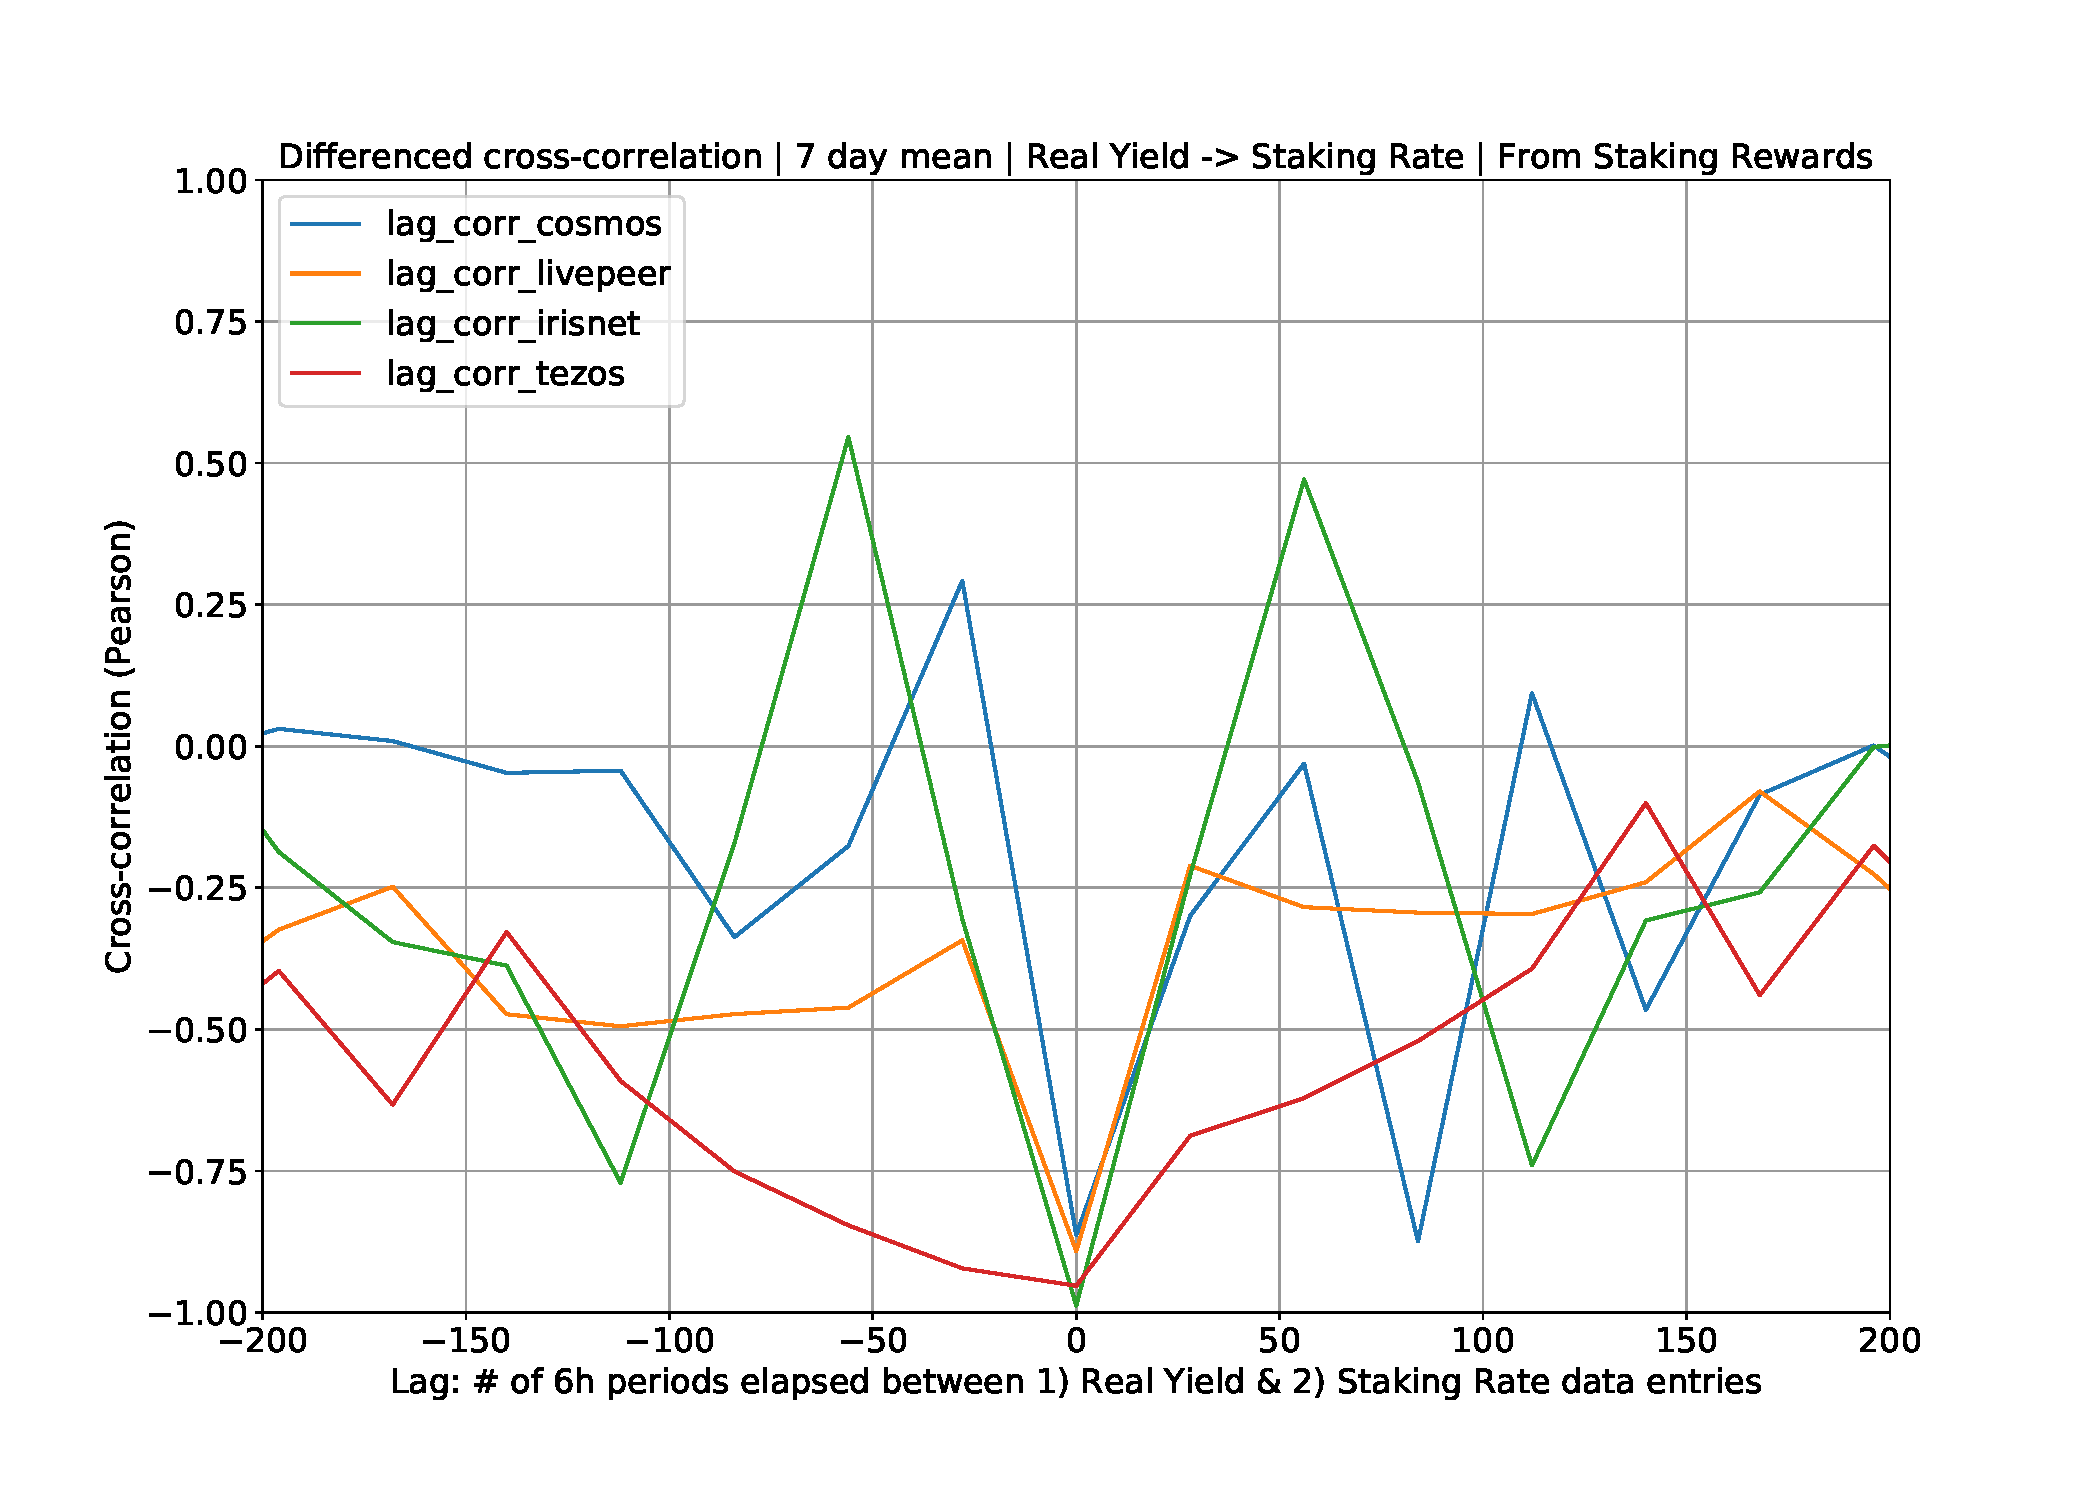
\includegraphics[width=1\textwidth]{graphs/CrossCorr_SR_DIF_7.pdf}
        \caption{7 day lump}
    \end{minipage}\hfill
    \begin{minipage}{0.5\textwidth}
        \centering
        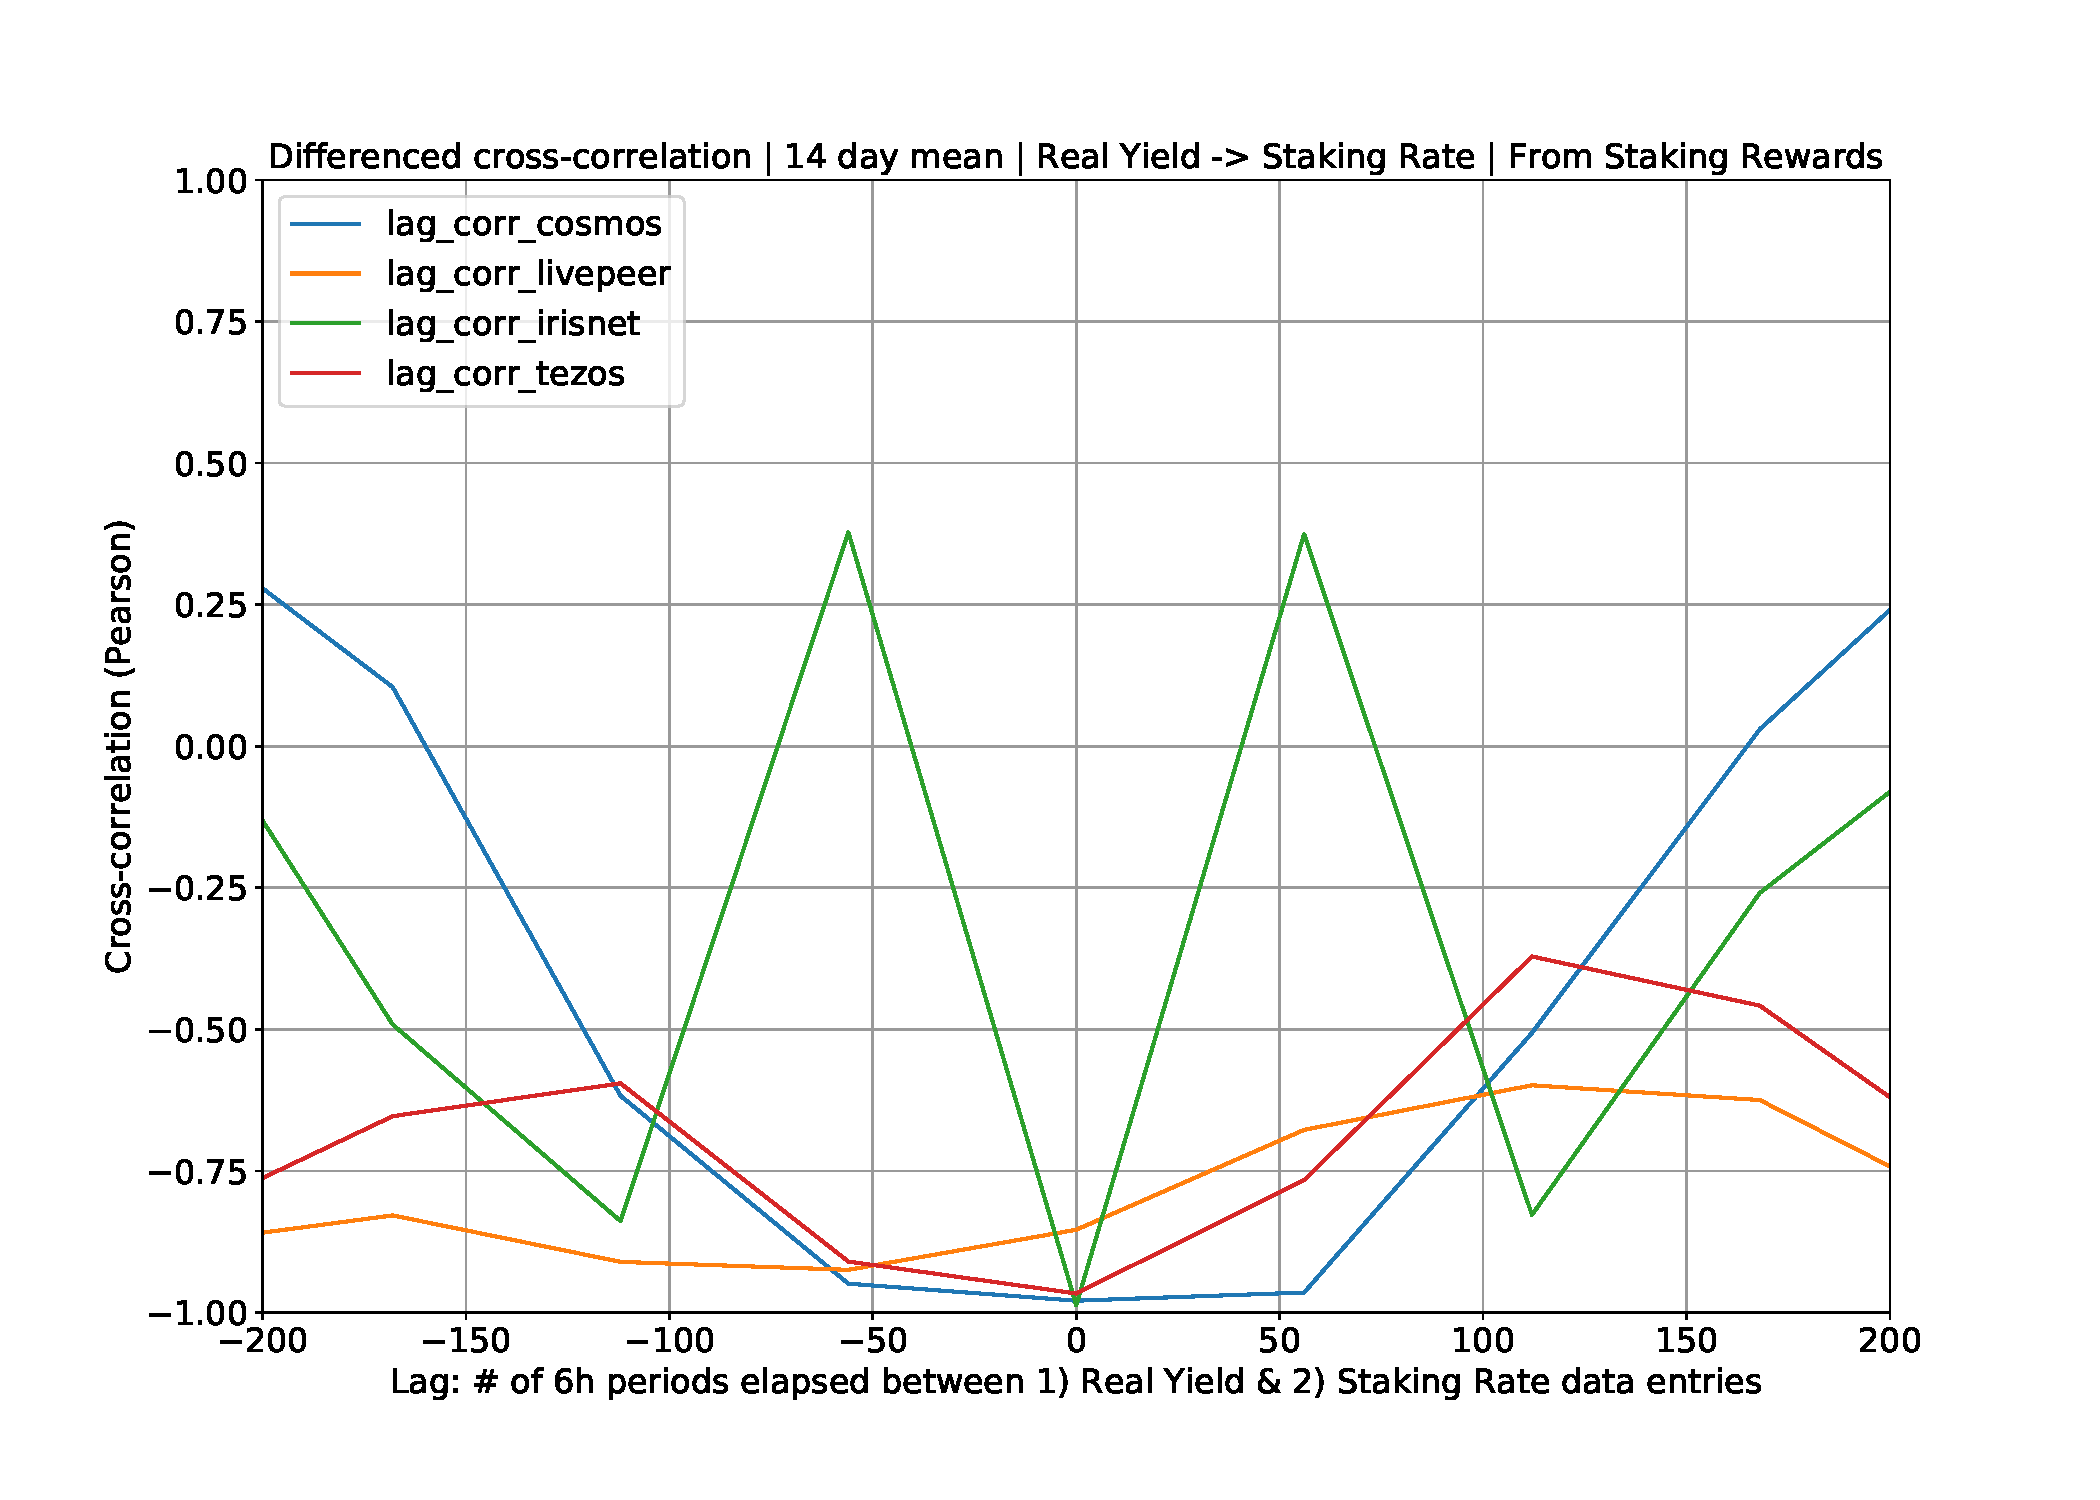
\includegraphics[width=1\textwidth]{graphs/CrossCorr_SR_DIF_14.pdf}
        \caption{14 day lump}
    \end{minipage}
    \begin{minipage}{0.5\textwidth}
        \centering
        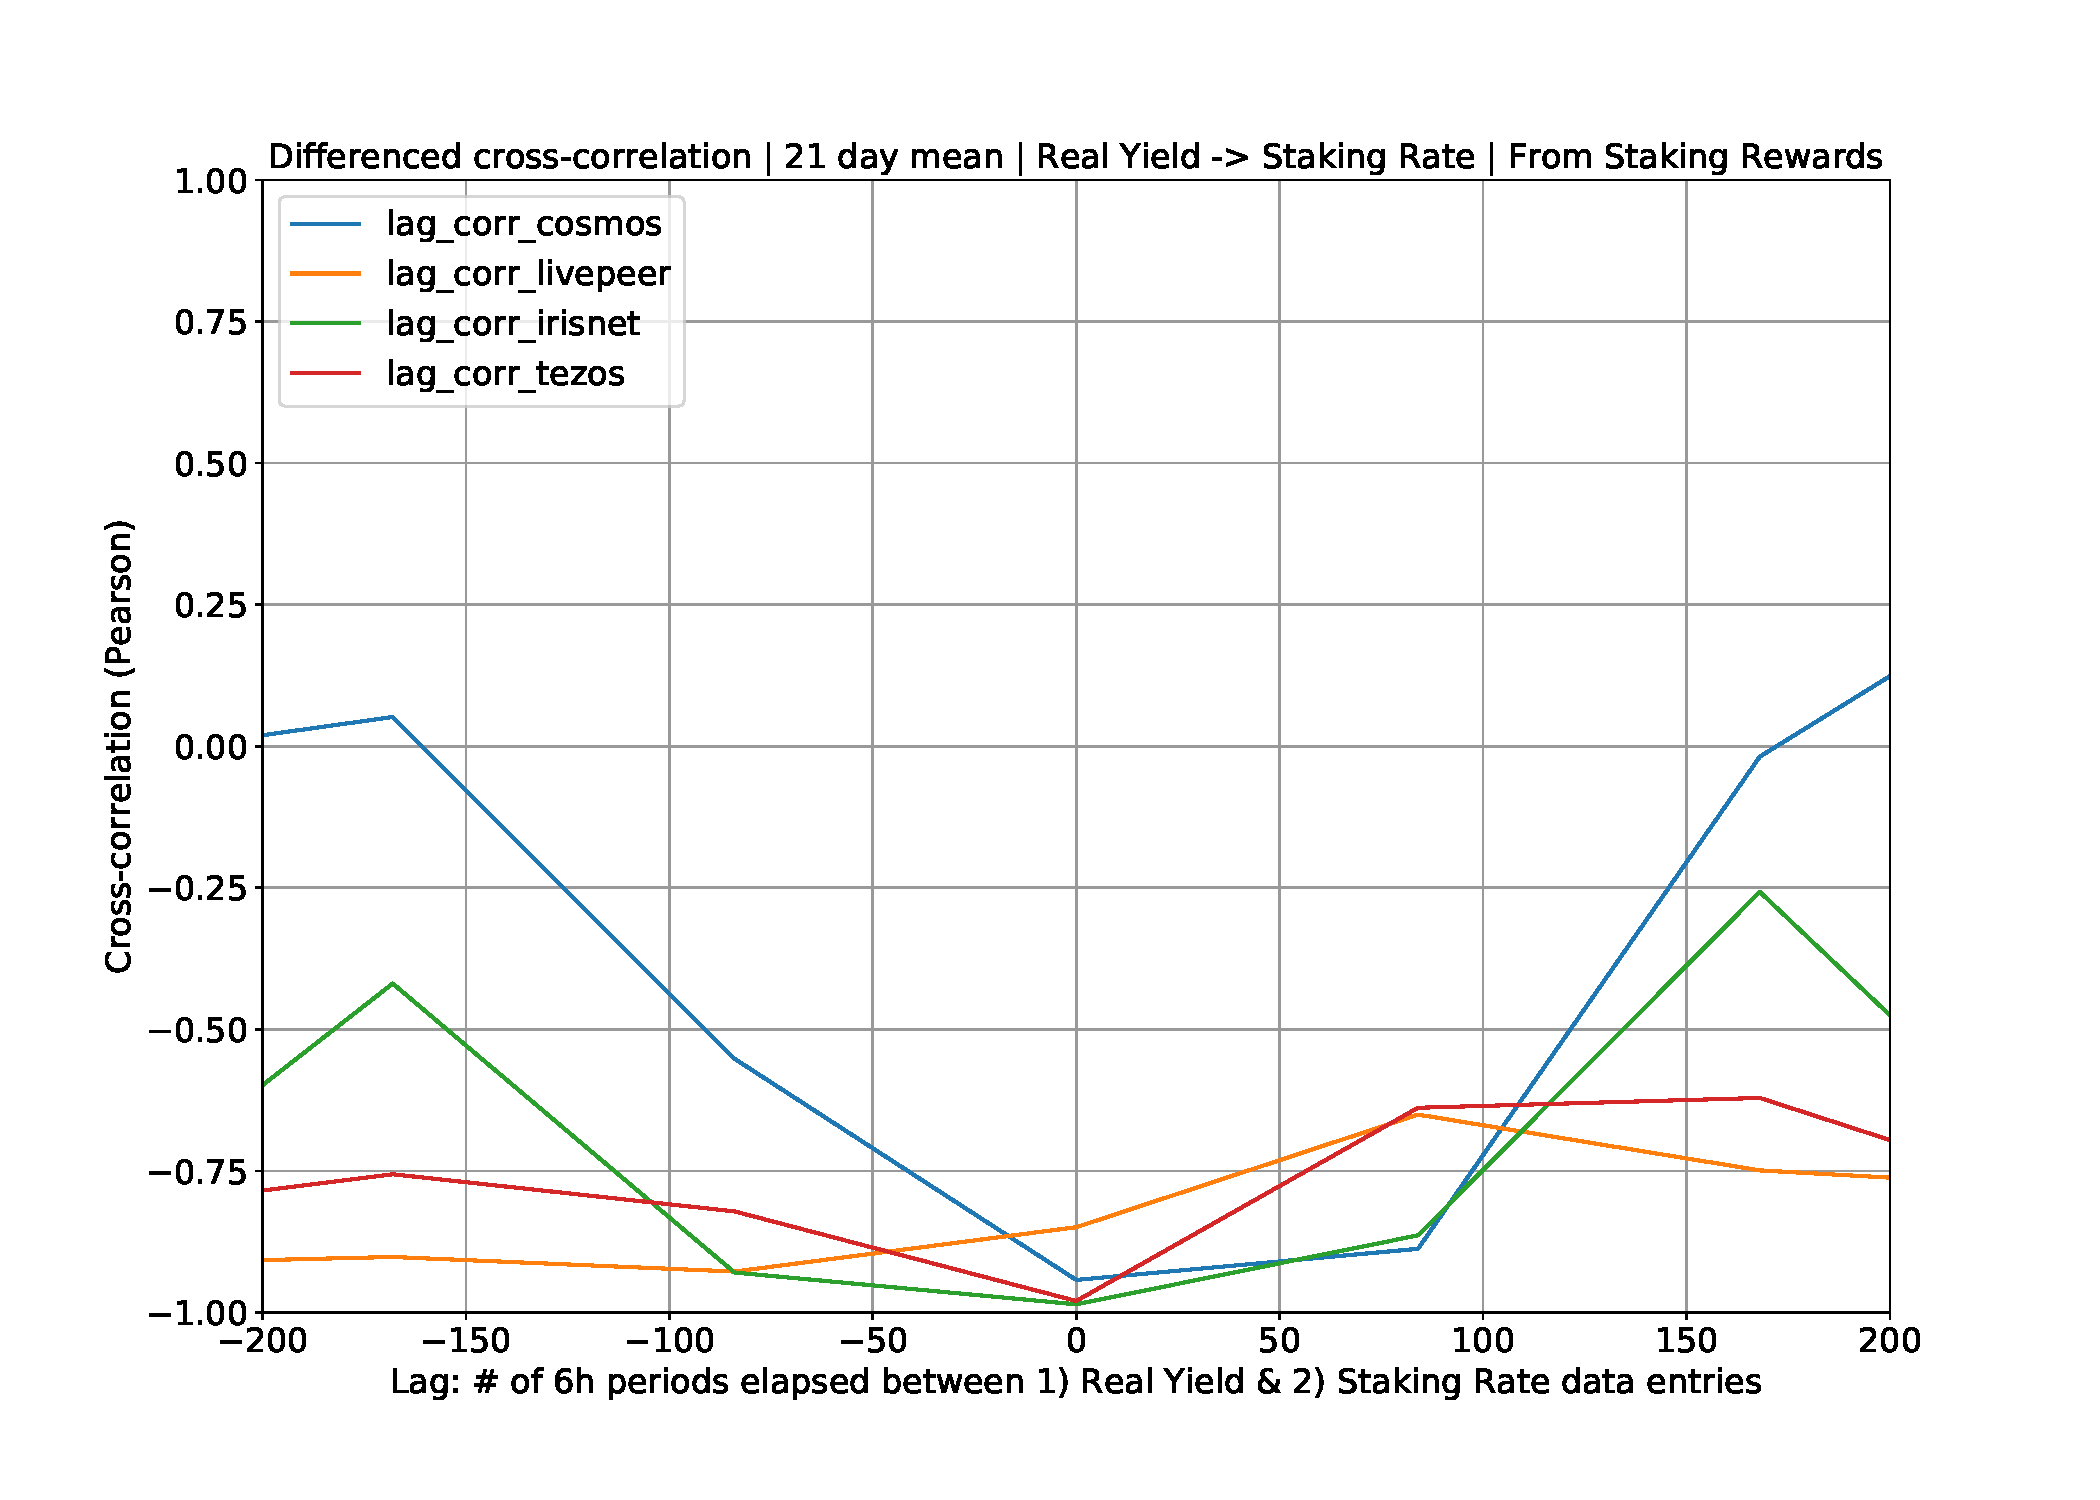
\includegraphics[width=1\textwidth]{graphs/CrossCorr_SR_DIF_21.pdf}
        \caption{21 day lump}
    \end{minipage}\hfill
    \begin{minipage}{0.5\textwidth}
        \centering
        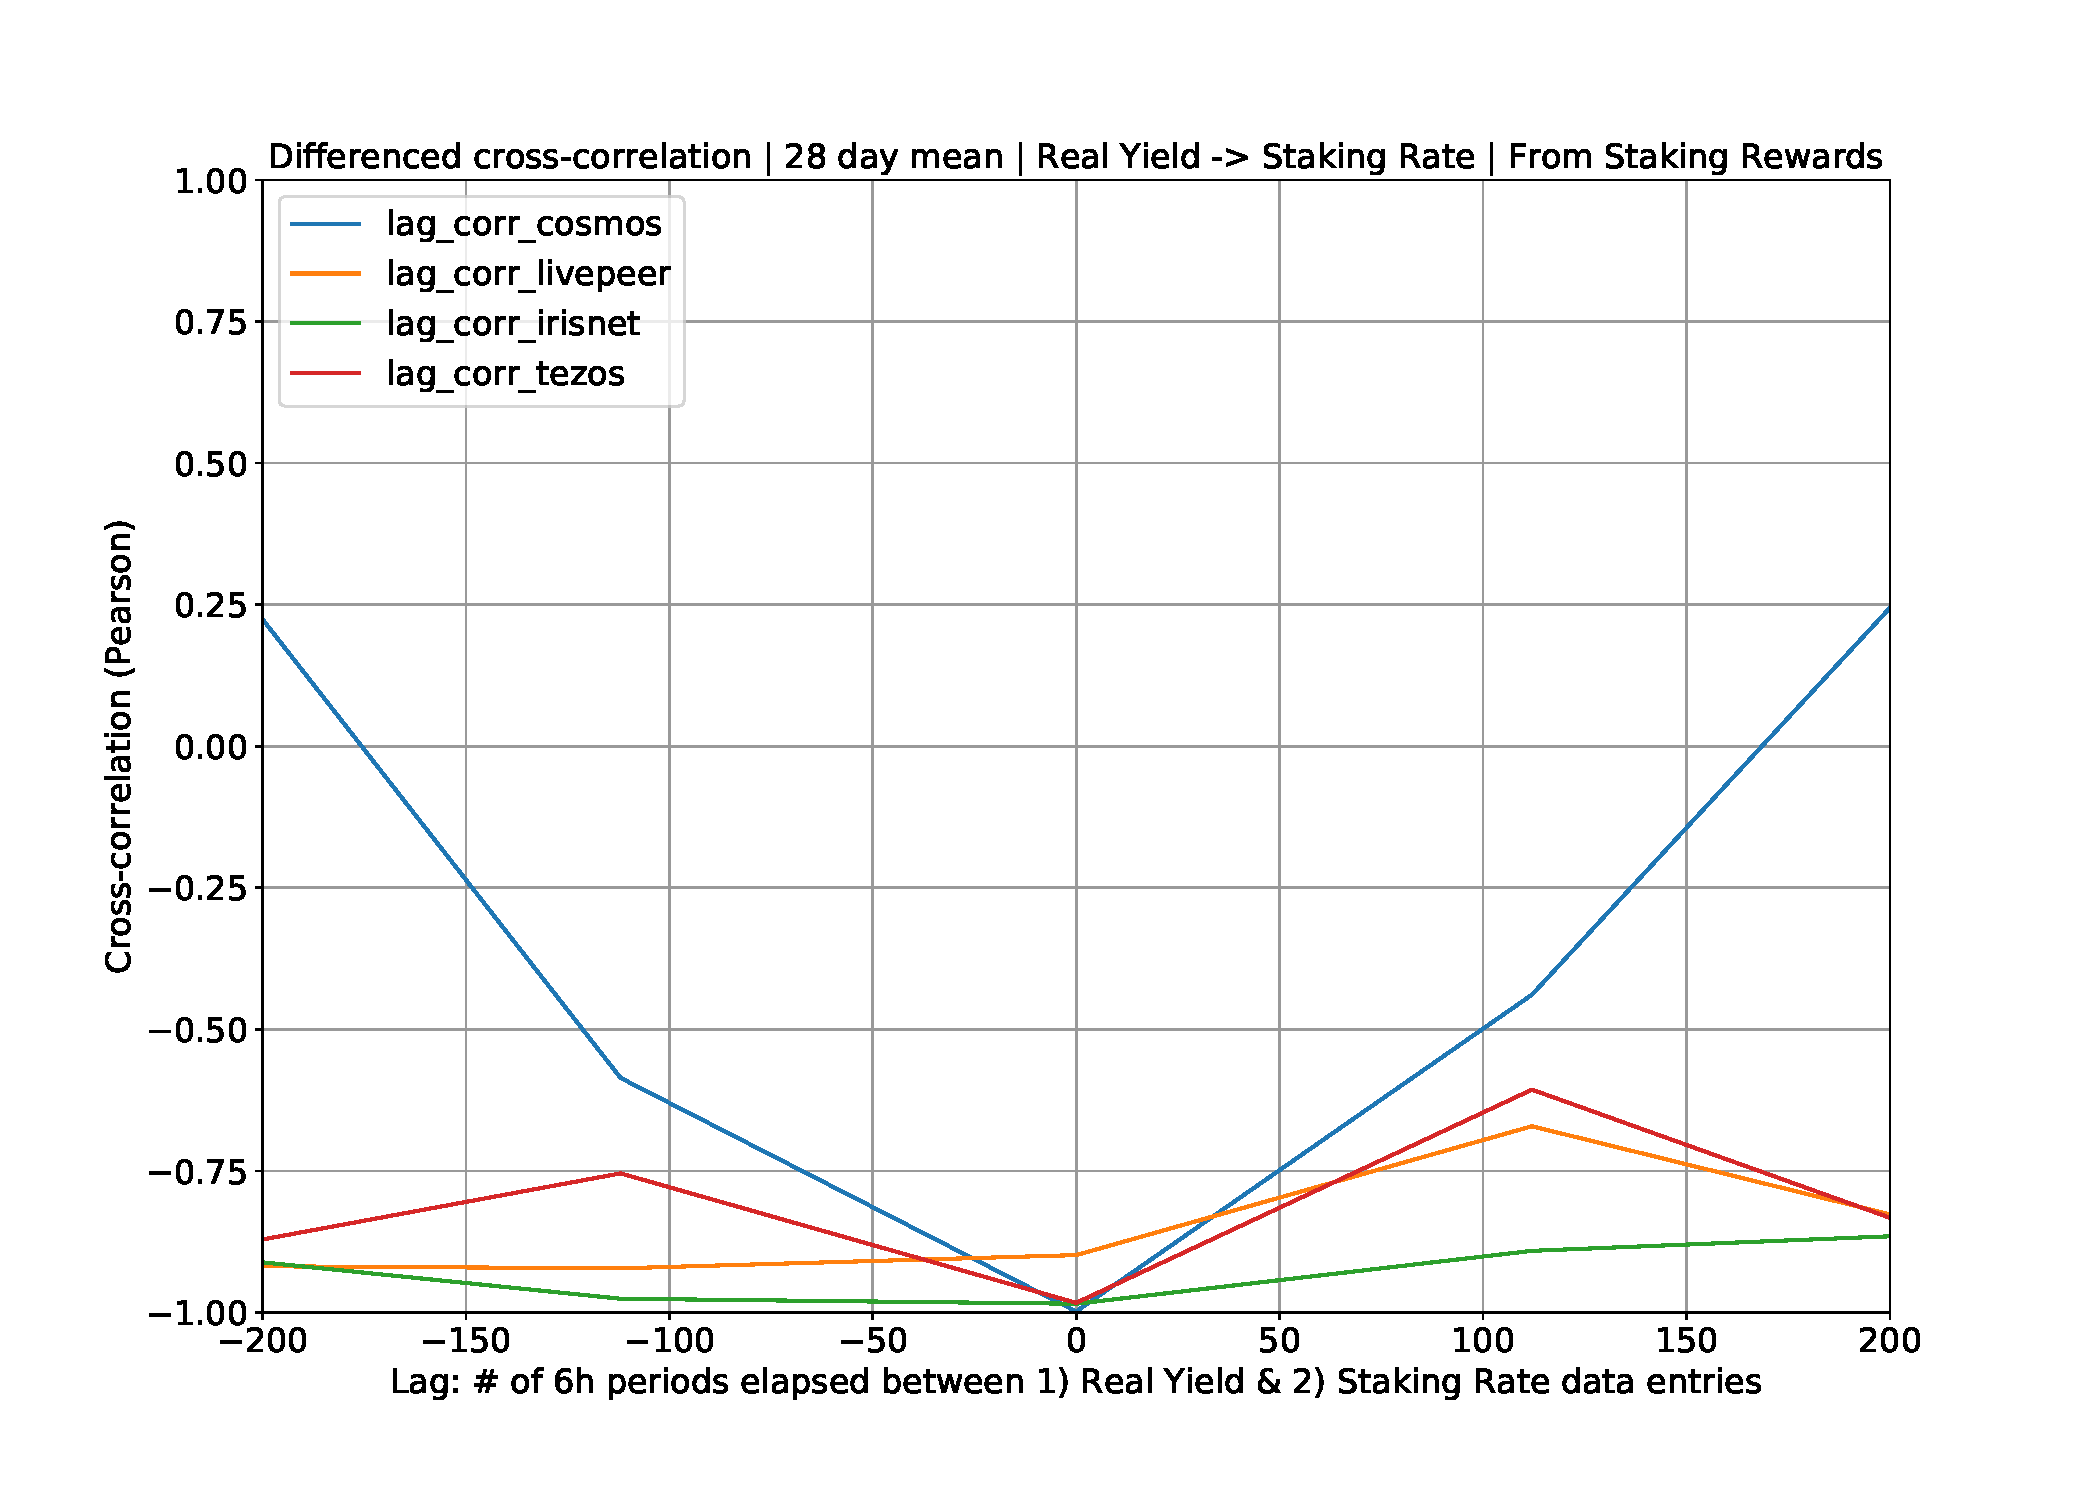
\includegraphics[width=1\textwidth]{graphs/CrossCorr_SR_DIF_28.pdf}
        \caption{28 day lump}
    \end{minipage}
    \caption{Cross-correlation of Real Yield and Staking rate, with a lag of $\pm50$ days instituted between the time series. Each graph shows a different lump size. Note that x-axis is expressed in 6h periods so 200 is equivalent to 50 days. Data from Staking Rewards.}
\end{figure}

\begin{figure}[h!]
 \centering
    \begin{minipage}{0.5\textwidth}
        \centering
        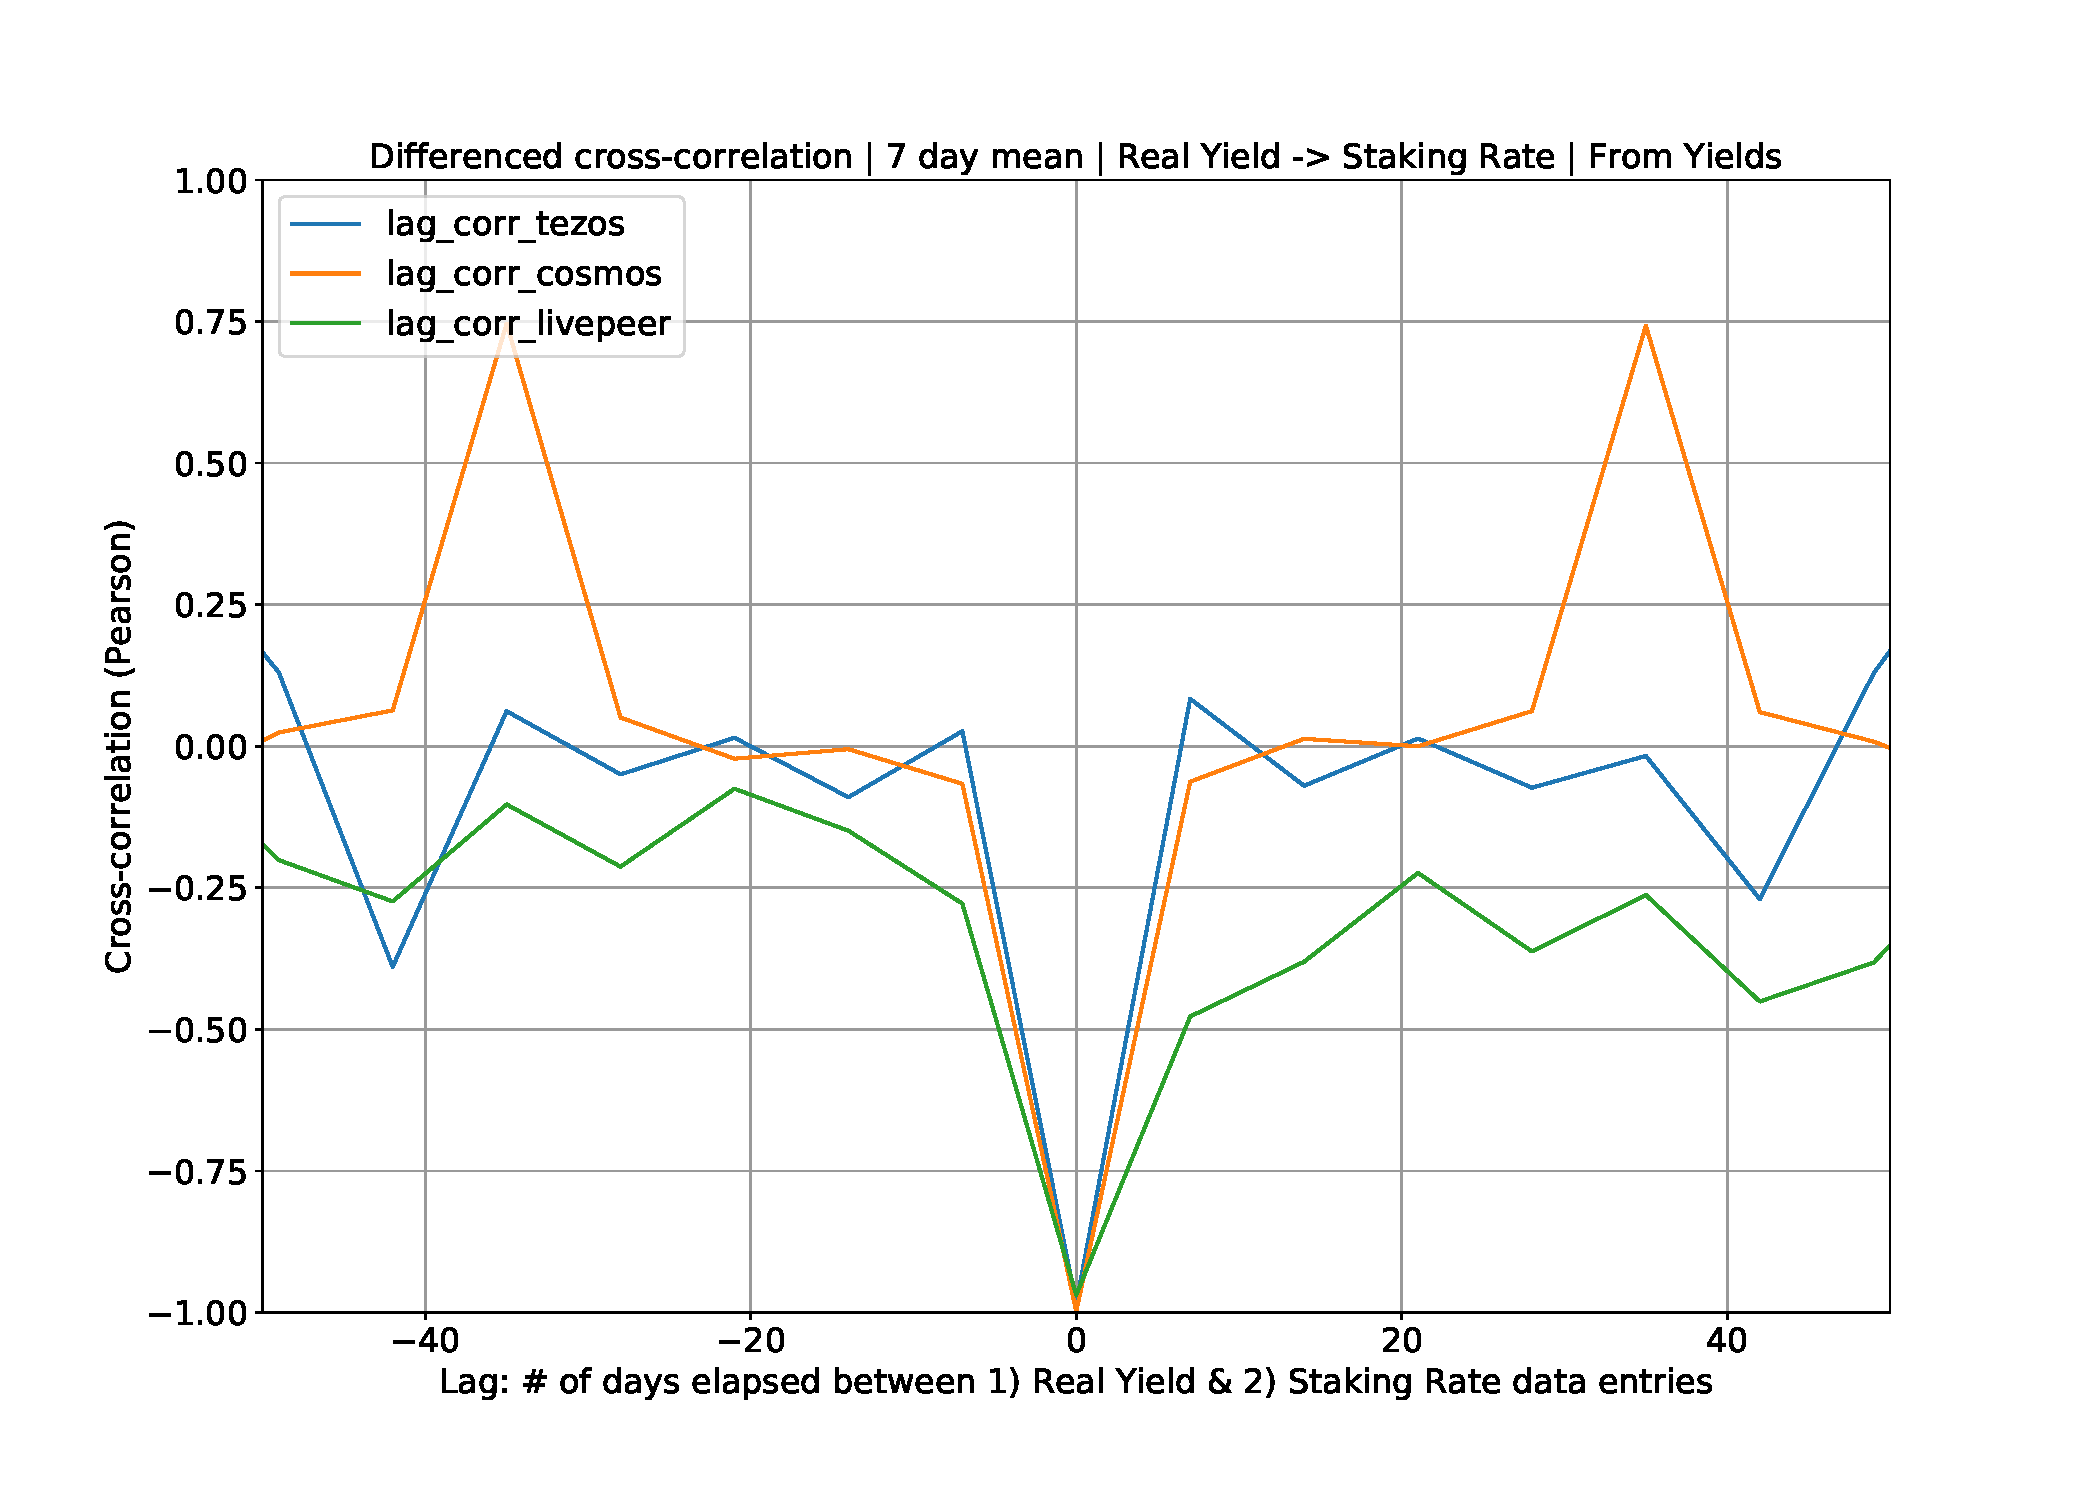
\includegraphics[width=1\textwidth]{graphs/CrossCorr_Yields_DIF_7.pdf}
        \caption{7 day lump}
    \end{minipage}\hfill
    \begin{minipage}{0.5\textwidth}
        \centering
        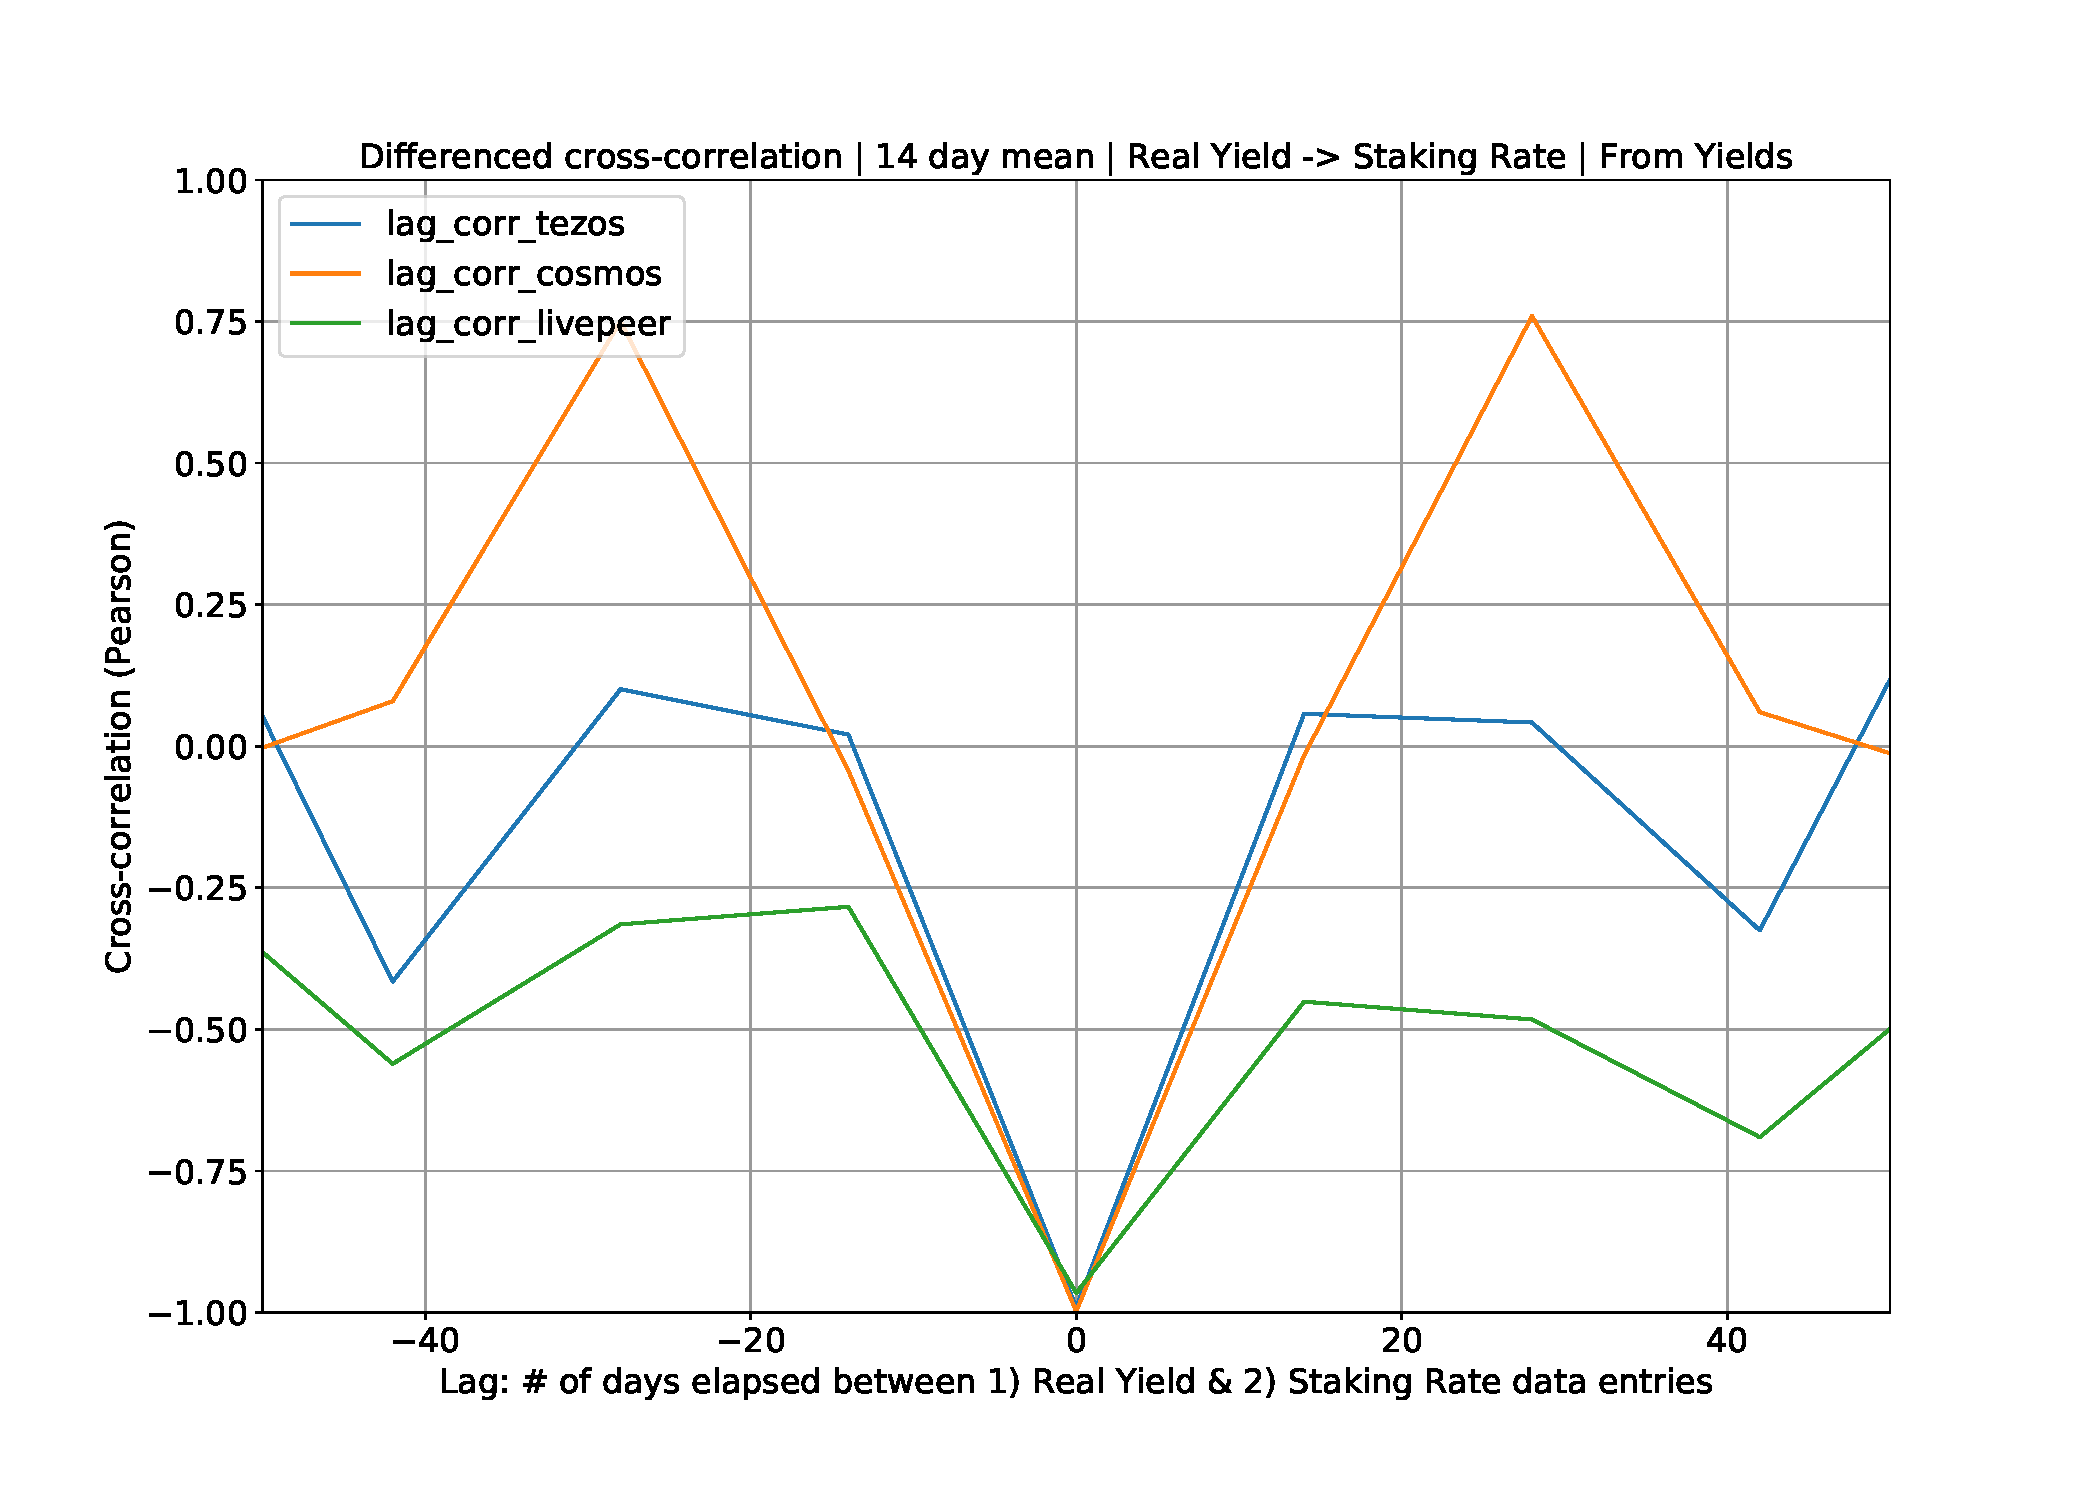
\includegraphics[width=1\textwidth]{graphs/CrossCorr_Yields_DIF_14.pdf}
        \caption{14 day lump}
    \end{minipage}
    \begin{minipage}{0.5\textwidth}
        \centering
        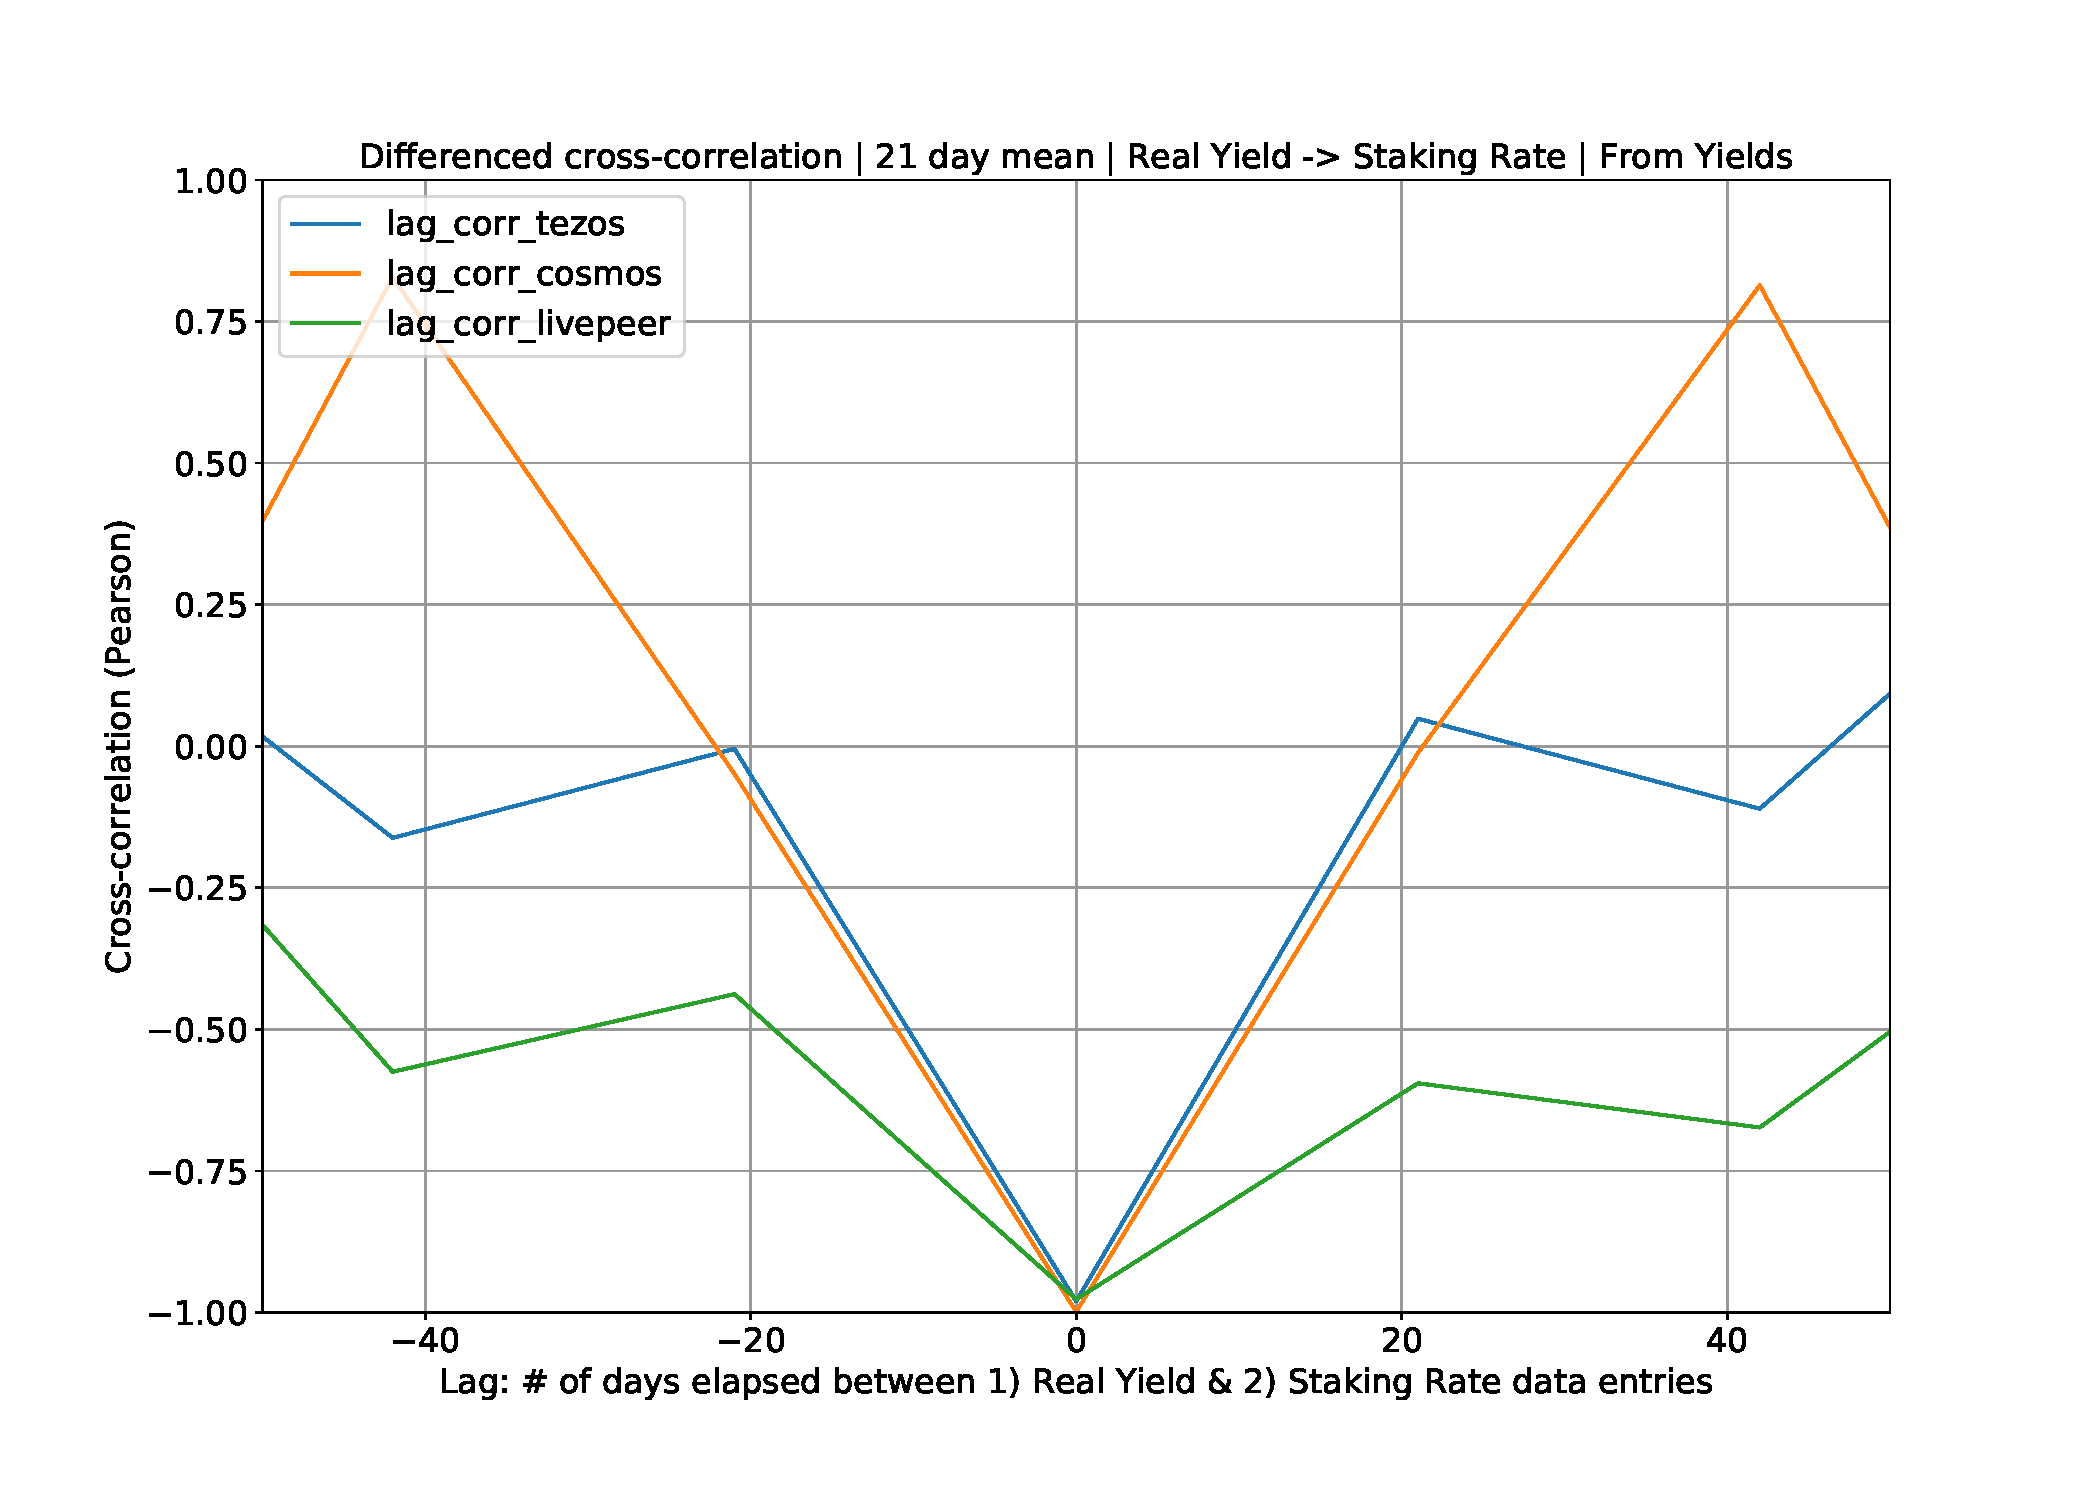
\includegraphics[width=1\textwidth]{graphs/CrossCorr_Yields_DIF_21.pdf}
        \caption{21 day lump}
    \end{minipage}\hfill
    \begin{minipage}{0.5\textwidth}
        \centering
        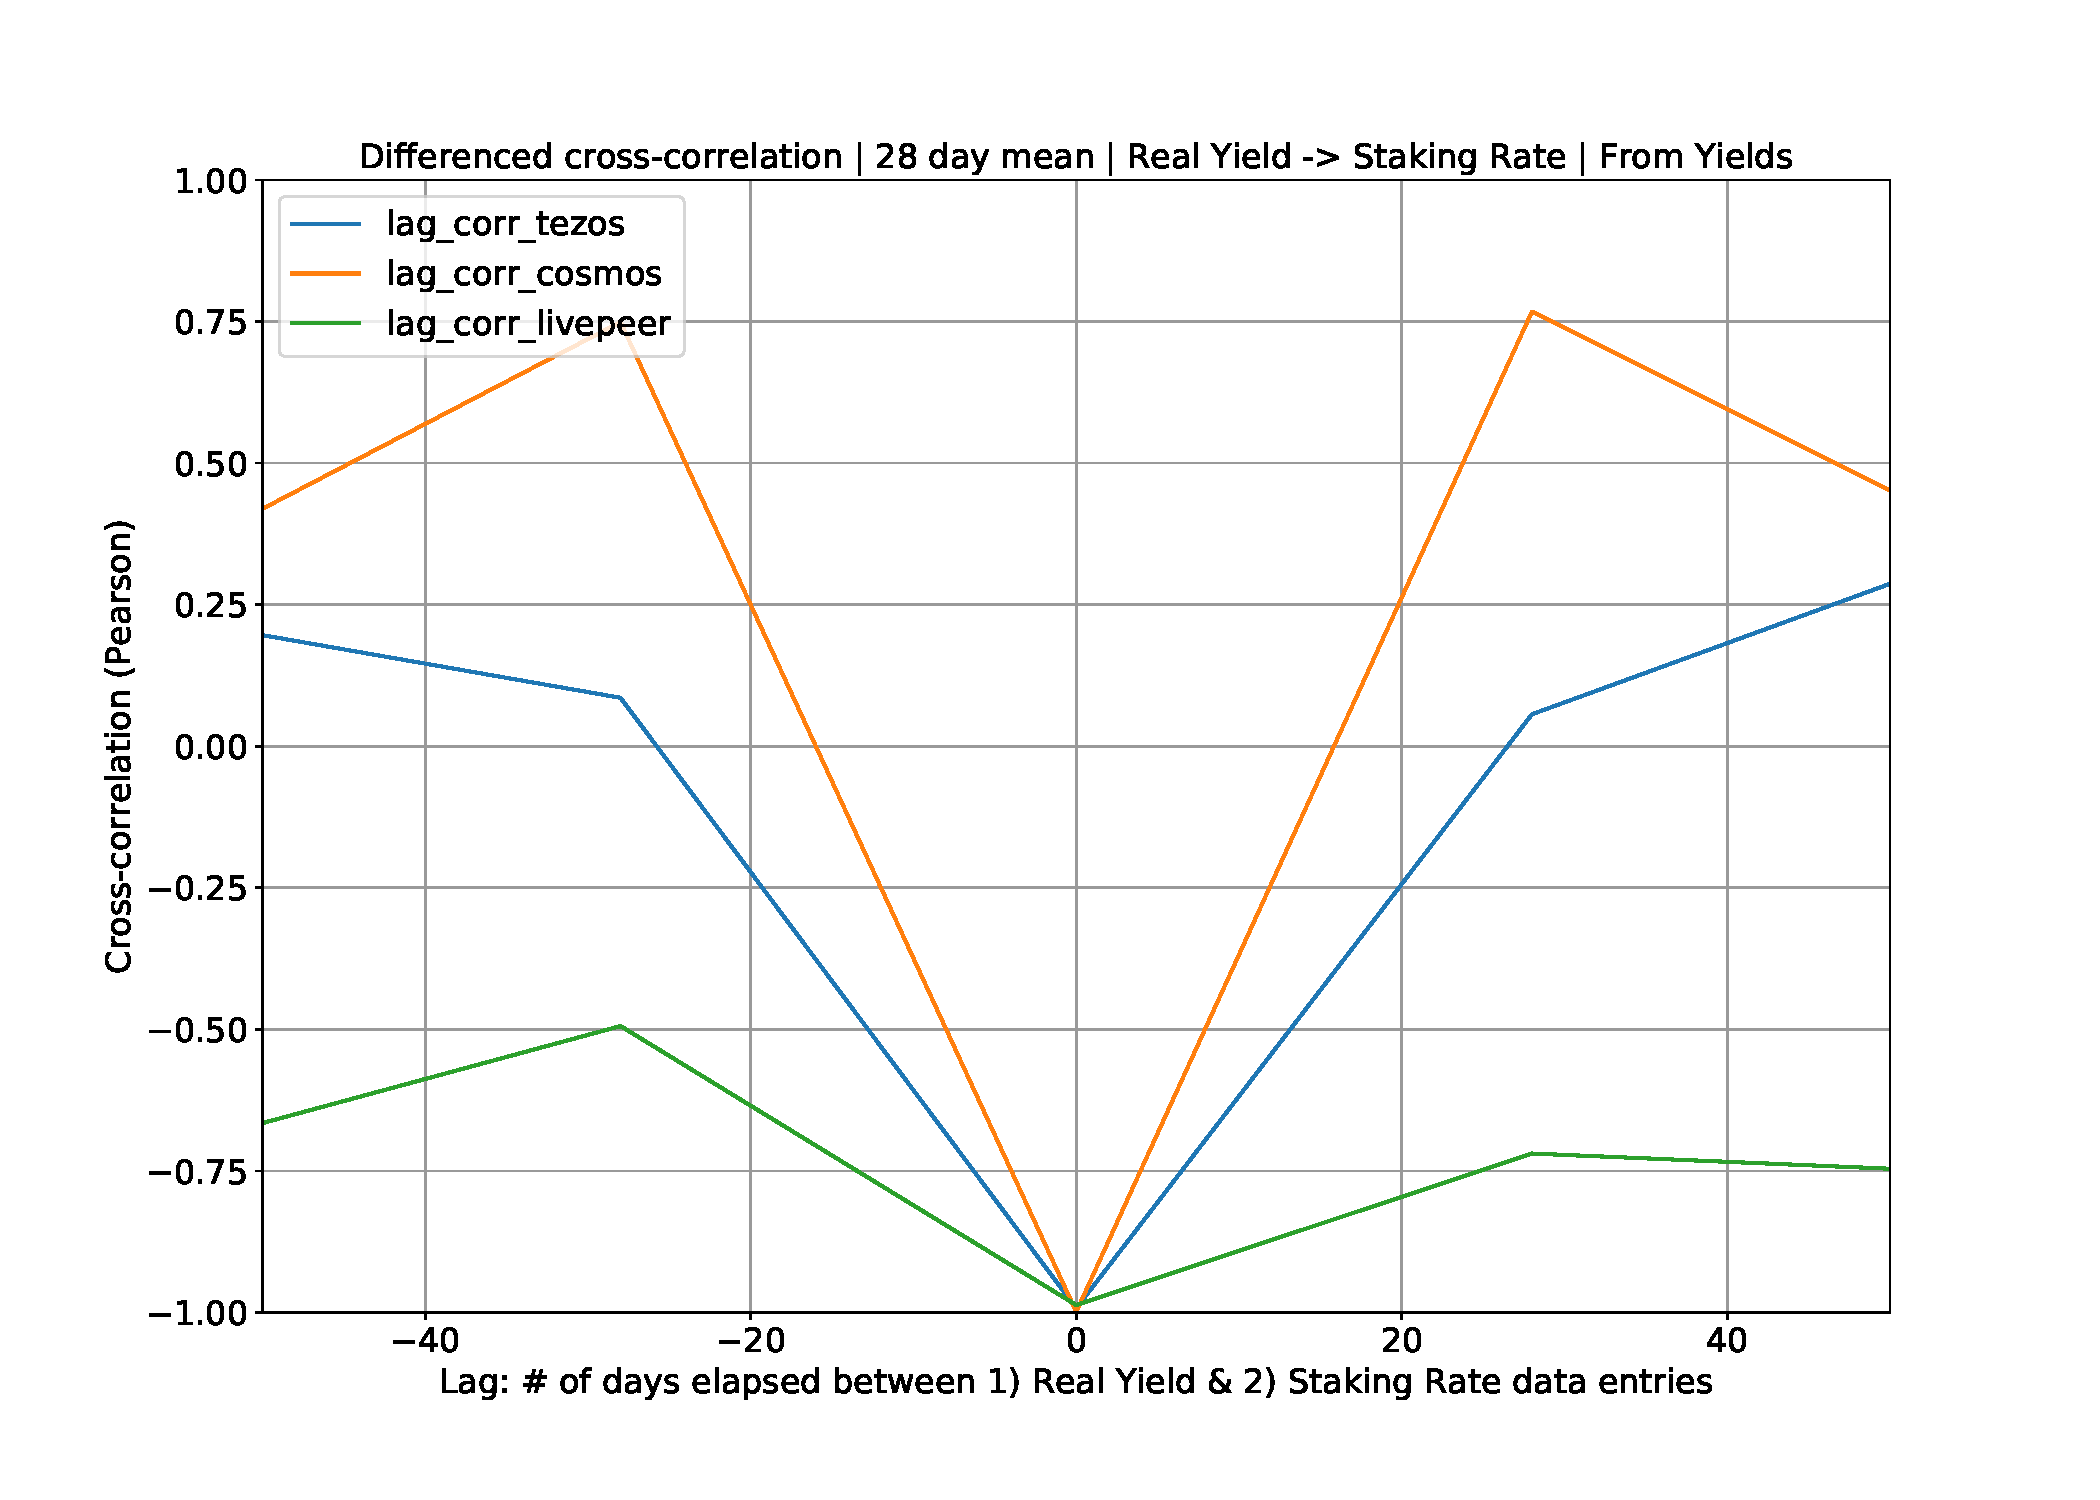
\includegraphics[width=1\textwidth]{graphs/CrossCorr_Yields_DIF_28.pdf}
        \caption{28 day lump}
    \end{minipage}
    \caption{Cross-correlation of Real Yield and Staking rate, with a lag of $\pm50$ days instituted between the time series. Each graph shows a different lump size. Data from Yields.}
\end{figure}

\subsubsection{Methodology}

The graphs in this section show the cross-correlation (Pearson) between the historical time series of the real yield and the staking rate, across a range of time-lags. All time series have been \textit{detrended} by training a linear regression model on the data, then subtracting the resulting trend from the data. All time series have also been \textit{differenced}. These two steps significantly reduce the autocorrelation and time-dependent structure of the data, granting the cross-correlations greater validity. Before the lagged cross-correlation was computed, each time series was `lumped' – using the 7, 14, 21 and 28 day mean to group the data. Each of these lump sizes are displayed and discussed individually.

\subsubsection{Analysis}

As expected, the cross-correlation is -1 when the lag is zero. This is the manifestation of the known dynamic mentioned in the previous section, where changes in the staking rate immediately impacts the real yield. We are interested in the reverse relationship – answering the question, `Does a preceding change in the real yield predict a change in the staking rate?'. This depends on human decision-making and behavior, and occurs over an unknown time lag, if at all. The right hand side of each graph (where the x-axis is positive) shows the results when the real yield data have been shifted, and so real yield readings are occurring `before' staking rate readings. This is where to look for evidence that the real yield might predict or cause the staking rate.
\\\\
It is notable that the cross-correlations in figures 6-9 (data from Staking Rewards) are largely \textbf{negative} or \textbf{too weak to be conclusive}. Indeed, there are no significant positive cross-correlations in any of the Staking Rewards results. In general, the smaller the lag, the stronger the negative correlation. In terms of network, Tezos and Livepeer display the strongest negative correlations. When the data is lumped using the 21 and 28 day means, all the networks besides Cosmos produce consistent negative cross-correlations across all lags.
\\\\
The Yields data (figures 11-14) do not have much in the way of strong cross-correlations, positive or negative, though there is a weak tendency towards the latter. The only exceptions are when the data is lumped using the 21 and 28 day means – Livepeer has strong negative cross-correlations across multiple lags, and Cosmos has a positive cross-correlation at a lag of around 30-40 days. 
\\\\
These results challenge established ideas about staker behavior – a widely-held assumption in staking protocol design is that lower earnings prompt stakers to reduce their stake size, which eventually increases average earnings for the remaining stakers in the next few subsidy rounds, thereby rebalancing the subsidy mechanism. In other words, protocol designers expect a causal relationship that mirrors the known, immediate dynamic (staking rate changing real yield), but perhaps more slowly. For this to be possible, we would at the very least need to see strong positive correlations between the real yield and staking rate once a lag is instituted. We can be agnostic about the magnitude of the lag, but even after 50 days, there is scant evidence that this rebalancing effect is happening in practice.
\\\\
The second implication of these results is that, in some cases, changes in the real yield is having the opposite effect as would be expected. The Staking Rewards data suggests that the collective staker reaction to lower real yields may be to increase their stake, and vice versa. This has 
\\\\
It's worth mentioning that the negative cross-correlations on display theoretically contain both the reaction of staking more in response to a lower real yield, and staking less in response to a higher real yield – but crucially, the latter necessarily occurs over with a time delay. It is not easy to disentangle these two dynamics within the results data. Nevertheless, we can make claims about specific data points – for example, let's look at the negative cross-correlation of -0.965 calculated for Cosmos, at a lag of 14 days (56 x 6 hour periods), in the 14 day lump, with Staking Rewards data. Given that Cosmos's unbonding delay is 21 days, this result is almost entirely explained by stakers depositing tokens, as opposed to withdrawing them. 
\\\\
More generally, a major unknown in these systems is the staker `reaction time'. Theoretically, a staker could respond to a changing real yield immediately, while another waits weeks for this change to evolve into a trend. Selecting a single lump size would introduce unacceptable experimenter bias into the results. Of course, 7, 14, 21, and 28 day lumps are not the full story, but they are a decent starting point. Lumps lower than 7 days seem unrealistic, since anecdotally, stakers are not known to change their stake size in response to hourly or daily changes to subsidies. The very weak correlations at the 7 day lump size demonstrate this. Lumps greater than 28 days run into sample size issues, where the total number of data points to run a Pearson correlation over drops to single digits.

\subsubsection{Interpretation with respect to two-phase model}

The notion that \textit{node operators can only be counted on for a reliable service if they are well compensated, or will quickly abandon the network} appears, so far, to be empirically unsubstantiated. None of the networks under examination, based on data from two independent sources, have experienced a shortfall of operators, nor are there any observable trends that correlate decreasing earnings with an increasing paucity of supply. The observable abundance of supply and lack of staker sensitivity to decreasing rewards appears to \textbf{derisk the two-phase model}, by undermining a possible objection – that relatively lower issuance in the early days of the network (see figure 1), will fail to attract or sustain a sufficient number of node operators. Remember that all the data in this study pertains to the very early months of each network's existence, so it is a reasonable model for the first few years of the NuCypher network.
\\\\ 
Why this seemingly unshakeable staker loyalty? One might attribute it to a prevalence of long-term investment strategies, deep pockets, large sunk costs, ideological commitment, or even irrational enthusiasm. Some stakers may respond to lower earnings by staking more because they hope to increase their individual subsidy – despite the fact this action will reliably lower everyone's revenue. Regardless of which underlying explanation one favours, there remains a strong case to flatten the minting schedule such that the earliest node operators do not capture a disproportionate share of the total supply.

\end{document}
